\documentclass[12pt] {report}

\usepackage[dvipsnames]{xcolor}
\usepackage[utf8]{inputenc}
\usepackage{adjustbox}
\usepackage [top=3cm, bottom=3cm, left=35mm, right=25mm] {geometry}

% Font style:
\usepackage{fontspec}
\setromanfont[
BoldFont=GARABD.ttf,
ItalicFont=GARAIT.ttf,
BoldItalicFont=GARA.ttf,
]{GARA.ttf}

\setsansfont[
BoldFont=GARABD.ttf,
ItalicFont=GARAIT.ttf,
BoldItalicFont=GARA.ttf,
]{GARA.ttf}

\setmonofont[Scale=1,
BoldFont=GARABD.ttf,
ItalicFont=GARAIT.ttf,
BoldItalicFont=GARA.ttf,
]{GARA.ttf}

\usepackage{pdfpages}


\usepackage[natbibapa]{apacite}

\usepackage{multirow}
\usepackage{array}
\usepackage{longtable}

\usepackage{graphicx}




\usepackage{graphicx} %package to manage images
\graphicspath{ {./images/} }
\usepackage[rightcaption]{sidecap}
\usepackage{wrapfig}


\usepackage{caption}
\usepackage{subcaption}

\usepackage{amsmath}
\DeclareMathOperator*{\argmax}{arg\,max}
\DeclareMathOperator*{\argmin}{arg\,min}

\usepackage{lscape}


\usepackage[utf8]{inputenc}
\usepackage[english]{babel}


\usepackage{chngcntr}   
\counterwithin{equation}{chapter}



\usepackage[labelfont=bf]{caption}
\captionsetup{labelfont=bf}

%\usepackage[demo]{graphicx}

\usepackage{hyperref}

\usepackage{indentfirst}

\title{Clustering three-way data structures: \protect \linebreak a time series approach}
\author{Gustavo de Oliveira Vital}
\date{\today}


%%%%%%%%%%%%%%%%%%%%%% BEGIN DOC %%%%%%%%%%%%%%%%%

\pagenumbering{roman}

\begin{document}

\date{}
\begin{titlepage}
\begin{center}

\begin{figure}[ht!]
    \centering
    
\includegraphics[scale=0.5]{images/FEP.PNG}
\end{figure}

\vspace*{0.7in}
{\LARGE \textbf{ {\scshape European Central Bank Speeches: A Sentiment Analysis Case Study}}}
\par
\vspace{0.4in}
{\large By}
\par
\vspace{0.4in}
{\large Gustavo de Oliveira Vital}
\par
\vspace{1in}
{\large Master Dissertation in Economics}
\par
\vspace{0.8in}
\end{center}
{\large Supervised by:} \\ 
\par
{\large João Manuel Portela da Gama}
\par
\vspace{0.10in}
%{\large Professor Y}
\vspace{1in}
\begin{center}
{\large \textbf{Faculdade de Economia}}
\par
\vspace{0.10in}
{\large Universidade do Porto}
\par
\vspace{0.2in}
{\large 2022}
\end{center}
\end{titlepage}


\thispagestyle{empty}

\newpage

\chapter*{Biographical note}



\addcontentsline{toc}{section}{Biographical note}
\setcounter{page}{2}

\newpage

\chapter*{Acknowledgements}








\addcontentsline{toc}{section}{Acknowledgements}
\setcounter{page}{3}



\newpage

\chapter*{Abstract}
This work intends to relate the press conferences of the European Central Bank, for a period from January 2005 to December 2020, with the macroeconomic scenario and with real European macroeconomic variables. As exposed by \cite[]{shapiro2020measuring, shapiro2021taking} and \cite[]{barsky2012information} it is possible to better understand what happens in the real economy from sentiment indices. This work follows \cite{shapiro2020measuring} when the author exposes the possibility of an economic index obtained by Natural Language Processing techniques through minutes and central bank reports, allowing a correlation with different macroeconomic scenarios. The methodology used includes processing techniques of Natural Language Processing and Sentiment Analysis. To relate the indices with macroeconomic variables, variable selection models are used (LASSO, Adaptive Lasso and Elastic Net). Furthermore, impulse response functions are obtained for a shock to the index and it is analyzed how the macroeconomic variables respond to a shock in the economic sentiment index.
\par
\vspace{0.5in}    
    
\noindent
{\bf Keywords:} Sentiment Analysis, Central Bank, Vector Autoregressive, Variable Selection Models.



  
\addcontentsline{toc}{section}{Abstract}
\setcounter{page}{4}


\newpage
\chapter*{Resumo}
Este trabalho pretende relacionar as conferências de imprensa do Banco Central Europeu, para um período de janeiro de 2005 a dezembro de 2020, com o cenário macroeconómico e com variáveis macroeconómicas reais europeias. Conforme exposto por \cite[]{shapiro2020measuring, shapiro2021taking} e \cite[]{barsky2012information} é possível entender melhor o que acontece na economia real a partir de indices de sentimentos. Este trabalho segue \cite{shapiro2020measuring} quando o autor expoe a possibilidade de um indice economico obtido por tecnicas de Natural Language Processing atraves de atas e relatórios de bancos centrais, permitindo uma correlação com diferentes cenários macroeconômicos. A metodologia utilizada engloba técnicas de processamento de Natural Language Processing e Sentiment Analysis. Para relacionar os indices com variaveis macroeconomicas, se faz o uso de modelos de seleção de variaveis (LASSO, Adaptive LASSO e Elastic Net). Ainda, são obtidas as funções de resposta ao impulso para um choque no indice e analisa-se como as variaveis macroeconomicas respondem a um choque no indice de sentimentos economico.



\par
\vspace{0.5in}

\noindent
{\bf Palavras-chave:} Análise de Sentimentos, Banco Central, Vetor Autoregressivo, Modelos de Seleção de Variáveis.
\addcontentsline{toc}{section}{Resumo}
\setcounter{page}{5}


%Contents:
\newpage
\tableofcontents

\newpage
\listoffigures

\newpage 
\listoftables

\newpage
\pagenumbering{arabic}
\chapter{\textbf{Introduction}}  \label{introduction}
\pagenumbering{arabic}

Economic decisions, in particular monetary policies, are based on resolutions provided by central banks. These remedies, however, are not always obvious, especially for lay people. For example, central bank minutes often include much more information than appears at first glance, especially when a group of texts is taken into account for a conjunctive or structural analysis. Understanding a collection of texts can occasionally be very difficult for a human being; depending on the purpose of understanding, the analysis can involve thousands or even millions of pages. However, thanks to developments in computing, questions like these are increasingly likely to be resolved. For a better understanding and knowledge of what a text, or a series of texts (corpus), actually says or expresses, techniques and tools like Natural Language Processing (NLP) and text mining are being heavily used.\\

It is already possible to discover trends in search engines such as Google and Yahoo using text analysis to anticipate macroeconomic indicators or even increase the understanding of consumer behavior. In recent study, \cite{bholat2015text} considers that, although the advances made in the field of computing are significant, the applicability of text mining in the economy is still not used as it could be. In the same study, the authors present cases of applicability of text mining in the economic field, with examples in the job market or even explaining how Natural Language Processing techniques can be applied to economics.\\

An alternative approach of application still in the field of Natural Language Processing is the sentiment analysis. Basically, it is “the task of identifying positive and negative opinions, emotions, and evaluations” \cite[]{wilson2005}. Sentiment analysis allows extracting information that normally a human being would not be able to, due to the amount of text, or even the difficulty of recognizing unstructured patterns. Through sentiment lexicons, it is possible to classify whether a text, phrase or words has a positive, neutral or negative expression (polarity-based lexicon) -- or even assign scores to a text, phrase or word (valence-based lexicon). When working with a set of economic texts, it is possible, then, to assign scores so that feelings can be monitored in a temporal way.\\	

Another article written by \cite{NYMAN2021104119} considered the possibility of a sentiment index, based on social media and networks, for a measure of excitement or anxiety about the financial and economic situation. The index proposes to act as a proxy for market sentiment: bullish or bearish. The ratio of the index would then be compared against historical events and other financial indicators \cite[]{NYMAN2021104119}. The idea of sentiment indices does not come from \cite{NYMAN2021104119} -- authors have already presented the possibility of modeling the economy by including non-observable variables that can represent economic sentiment. Even though in studies such as \cite{barsky2012information, angeletos2013sentiments, akerlof2010animal, gennaioli2018crisis, bholat2015text} the idea of economic sentiments has already been presented; Previous studies \cite{shapiro2020measuring, shapiro2021taking} presented the idea of an index of sentiments coming from Natural Language Processing techniques, where the index presents a boost to economic activity.\\

Gradually, Natural Language Processing techniques and tools have been increasingly used with implementations in the economic field. It is not difficult to find correlations between macroeconomic variables and sentiment analyzes extracted from the media, economic newspapers or magazines \cite[]{ostapenko2020macroeconomic, NYMAN2021104119} or even from speeches or parliamentary hearings of central banks \cite[]{fraccaroli2020central, shapiro2020measuring, shapiro2021taking}.\\

The examination and investigation of how textual patterns supplied by the European Central Bank can point to and connect with conjunctural and structural moments of the economy is the major goal of this work. From the speeches of the European Central Bank, an index of economic sentiment was elaborated that can reflect what the economic scenario goes through -- that is, the reflection of the economy from the point of view of the economic speeches of the European Central Bank. The use of Natural Language Processing techniques in the economics field can be very advanced and useful for a better understanding of what central banks are actually indicating (through textual documents), and not just reduce the central bank's indication based on its own resolutions. Language Processing techniques are being used more and more to capture patterns that are practically imperceptible to the human eye.\\

The greatest relevance and contribution of this work is the use of the speeches of the European Central Bank as an indicator of economic sentiments. From this point, it will be possible to compare the results obtained with previous correlated works in the literature so that an “asymptotic” relationship is expected in terms of results -- in terms of counter intuition, the objective of this work is to corroborate the indicated literature.\\

The chapter \ref{chapter:lit} presents the bibliographic review of this work and exposes the main works used as a reference for this bibliography. The chapter exposes the point of view of \cite{shapiro2020measuring, shapiro2021taking} articles that made use of Natural Language Processing and Sentiment Analysis techniques. Also, other articles \cite{barsky2012information, angeletos2013sentiments} are exposed that work with the \textit{concept} of feelings in an economic scenario, even when considering a general equilibrium scenario.\\

The \ref{cap:methodology} chapter presents the review and introduction of the reference methodology, related to the Natural Language Processing parts and lexicons. Two fundamental lexicons are exposed and used in this work -- VADER \cite[]{hutto2014vader} and LM-SA-2020 \cite[]{lmdata}, the first lexicon being a valence-based lexicon and the second a polarity- based lexicon, economically grounded. Still, concepts of Natural Language Processing and Sentiment Analysis are defined.\\

The \ref{cap:results} chapter presents the result of the present work. This chapter addresses the case study carried out. Using the speeches of the European Central Bank as a basis, two studies are carried out: in the first, models of selection of variables are estimated to infer whether indices of economic sentiments based on NLP would be statistically significant for the estimation of economic variables; and in the second study we estimate the responses of the impulse response functions given a shock in sentiment indexes using an Autoregressive Vector -- this would make it possible to understand how the estimated economic variables would behave when a ``variation'' of sentiments occurs in the economic scenario.\\

The work ends with the fifth chapter, highlighting the final considerations of the dissertation and the conclusions regarding what was done.


\chapter{\textbf{Literature review}}  \label{chapter:lit}

According to \cite{chowdhury2003} ``Natural Language Processing (NLP) is an area of research and application that explores how computers can be used to understand and manipulate natural language text or speech to do useful things''. In order to build the right tools and techniques to enable computer systems to comprehend and manipulate natural languages to carry out specified tasks, researchers in natural language processing seek to learn about how people interpret and use language.\\

Working with quantitative and qualitative data simultaneously is one of the benefits of using documents, texts, and minutes \cite[p. 1]{bholat2015text}. Even while these types of studies have a wide range of applications, they have only recently been employed in economics despite the fact that working with both types of data makes it possible to conduct research and draw statistical inferences that are not achievable with simply structured data. In this way, it would be possible to have a better understanding of what happens in the economic scenario behind models that we work with NLP -- understanding feelings and emotions of economic agents has always been a goal of science, whether for a better understanding of its uses or even in terms of behavior of the consumer.\\

In a recent study, \cite{shapiro2020measuring} presents new evidence that incorporate NLP techniques into economic science. According to the authors, it was possible to obtain a sentiment index that matched the Michigan Consumer Sentiment Index (MCSI)\footnote{\url{http://www.sca.isr.umich.edu/}}, from economic articles and assessed financials. In terms of methodology, it would then be possible to obtain an index of consumer sentiment through selected journals and textual sentiment analysis techniques. Two studies were proposed: first, it would be analyzed whether the sentiment index elaborated by the authors would be a good predictor variable for real economic variables. For this exercise, the authors used three models of variable selection as a methodological approach: a LASSO, an Adaptive LASSO and a Group LASSO. The variable selection models showed that the sentiment index is significant in the predictor aspect, even when compared to the Michigan Consumer Sentiment Index, the LASSO Group points out the authors' index (based on sentiment techniques) as superior in some models ``Specifically, at least one of the LASSO versions prefers the news sentiment measure in forecasts of employment, output (IP), inflation, the real rate (FFR), and the S\&P 500'' \cite[p. 26]{shapiro2020measuring}. The economic variables used for this study were: employment, output, inflation, the real rate, the consumption, the S\&P 500, the MCSI, and the Conference Board's Consumer Confidence index, in addition to the authors' sentiment index.\\

In a second exercise carried out by the authors, it was analyzed how economic activity would react to a positive shock in the sentiment index. Unlike the conventional method (from an autoregressive vector), the impulse response functions were obtained through local projections \cite{jorda2005estimation} (similar to VAR, but with a less restrictive approach). The results obtained demonstrate that a positive shock in the sentiment index would lead to a slight increase in consumption, in the economy's output, in the real interest rate and in the price level. In addition to these results, impulse responses were also estimated for the Michigan Consumer Sentiment Index and the Conference Board's Consumer Confidence index (CBCI). When analyzing the responses of economic activity to the MCSI, the economic variables (with the exception of the interest rate that responds positively) were not statistically significant. When analyzing the responses of the economic variables to a CBCI choue, the results are similar to the results obtained with the authors' sentiment index -- the responses of the economic variables are statistically significant and point to a slight increase.\\

From economic articles, then, it is possible to analyze and better understand the economic situation. The extraction of a sentiment index through NLP techniques also saves the time and funds needed to obtain an index of this content. With the passage of time, the NLP techniques will evolve, allowing, thus, an improvement in the computational field and in the part of sentiment analysis applied to the economy.\\

In another article, \cite{shapiro2021taking} analyzes Federal Reserve deliberations from NLP techniques to estimate central bank preferences. In other words, it would be possible to estimate the objective function of some generic central bank from its speeches or internal meetings.\\

Based on the estimation of the central bank's loss function, the results showed that the inflation target for the analyzed period (2000-2011) was approximately 1.5\%. With this result, it is possible to perceive that, as everything indicates, the value of the inflation target would be, therefore, significantly below what the surveys of inflation expectations indicated in the period -- for the long term. However, it has been documented \cite[p.32]{shapiro2021taking} that the position of certain members of the Federal Open Market Committee\footnote{Where the speeches come from.} have sometimes stated that an inflation target of 1.5\% seemed consensus at least until 2009 -- after this period, the inflation target value would be 2.0\%.\\

The article also finds that the ``negativity'' of the FOMC is most affected by economic growth and financial conditions. This statement is supported by \cite{walsh2003speed}, which addresses how central banks end up focusing more on economic growth and \cite{coibion2011monetary} which raises this hypothesis based on empirical estimations of the Taylor rule. In a previous work, \cite{thornton2011does} has already pointed out that the FOMC ends up focusing more on the issue of ```growth in output', and not sustainable employment, the unemployment rate, or any concept of slack, as part of their policy directive from 1979 through 2008'' \cite[p.34]{shapiro2021taking}. A question also raised by the article was how financial variables would behave in the face of FOMC speeches. \cite{bernanke2001should} points out that monetary policy should not, for example, respond to a change in asset prices. Having an opinion that supports this study, former Fed Vice President Don Kohn says that the Fed does not respond to asset prices \cite{kohn2006monetary, kohn2009monetary}.\\

On the other hand, a study by \cite{peek2015should} presents financial variables as good predictors of the Fed's interest rate, when these are incorporated into a Taylor rule that takes into account financial instabilities. Finally, \cite{cieslak2021economics} points out that both a stock market crash and a real negative stock market return affect FOMC discourses, and thus become predictive variables of the Fed's interest rate.\\

In another article, to better investigate consumer behavior and sentiment, \cite{barsky2012information} developed two fundamental strategies: the estimation of a new Keynesian DSGE, and the estimation of several VAR models. Through the answer of a question, ``Turning to economic conditions in the country as a whole, do you expect that over the next five years we will have mostly good times, or periods of widespread unemployment and depression, or what?'' \cite[p.1347]{barsky2012information}, the authors created a variable (E5Y) so that this is the percentage of favorable answers to the question minus the percentage of negative answers to the question plus 100. The authors did the same, then, to a horizon of 12 months ahead, and called the variable E12M, in order to better understand how expectations would vary in different future timeframes. Also, they create the expected personal financial (PFE) variable, according to the answer ``Now looking ahead -- do you think that a year from now you (and your family living there) will be better off financially, worse off, or just about the same as now?'' \cite[p.1371]{barsky2012information} and finally create a consumer expectation index (ICE) according to the equation:

\begin{align} \label{eq:ice}
    ICE = \frac{PFE + E12M + E5Y}{4.1134} + 2.0
\end{align}

another index, the consumer sentiment index (ICS) is developed from a variation of the equation (\ref{eq:ice}):

\begin{align} \label{eq:ics}
    ICE = \frac{PFE + E12M + E5Y + DUR + PFP}{6.7558}
\end{align}

where in the equation (\ref{eq:ics}) DUR represents ``wheater or not it is currently a good time to buy `large household items''' \cite[p.1372]{barsky2012information} and PFP is identical `` to PFE, except that PFP respondents to compare their current financial situation relative to one year ago''\cite[p.1372]{barsky2012information}.\\

Based on this interest in a possible sentiment index, the authors estimated VAR models in order to understand how this index would behave if modeled against variables of economic activity. The authors demonstrate from impulse response functions that economic variables such as consumption would have, given a positive shock on the sentiment index, a temporary positive change. The same happens when analyzing the output of the economy.\\

The authors go further and implement a new Keynesian DSGE model incorporating into the model an ``animal spirit'' effect interpreted as ``noise innovations in the signal about productivity growth''\cite[p.1353]{barsky2012information} and trust, represented by E5Y. Assuming that agents observe the technology level from period to period, a noisy signal of the growth rate can be observed:
\begin{align*}
     s_t = g_t + \varepsilon_{s,t}
\end{align*}
where $g$ is an AR(1) stationary process of growth and the shock $\varepsilon_{s,t}$ is interpreted as the animal spirit shock. E5Y in turn is modeled according to the autoregressive process:
\begin{align*}
     E5Y_t = (1 - \rho_e) + \rho_e E5Y_{t-1} + u_t
\end{align*}
where $u_t$ represents the innovation in confidence\footnote{$u_t$ is also modeled as an autoregressive process of order 1. For further explanation, see \cite[p.1354]{barsky2012information}}.\\

The objective of the DSGE estimation was to compare the results of the impulse responses of an anial spirit shock with the results obtained in the VAR models. This ends up having repercussions on another question: ``why are confidence innovations prognostic of future movements in economic activity''\cite[1356]{barsky2012information}? The estimation results corroborate previous studies \cite{rotemberg1997optimization, christiano2005nominal} on the topic.\\

%
%\begin{figure}[!h]
%    \centering
%    \caption{Impulse response of a positive news sentiment shock on economic activity}
%    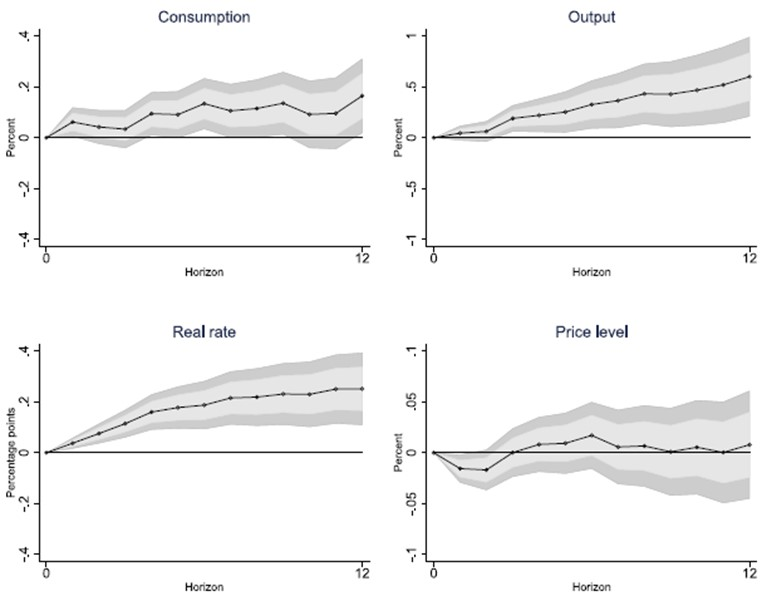
\includegraphics[width=.8\textwidth]{images/image1.jpg}
%    \caption*{Source: \cite[p.16]{shapiro2020measuring}}
%    \label{fig:my_label}
%\end{figure}














In order to complement the literature of sentiment analysis in economics, \cite{ostapenko2020macroeconomic} contributed analysing “how the change of tone or topic in newspaper affects the macroeconomy”. The author transformed articles from newspaper (employing a topic model and vector representation of documents with clustering) into time series and based on this time series, evaluated the sentiment of each article. On occasion, the article demonstrated that given a new shock in the sentiment of the articles, it could mean an increase over the long run, in output and consumption – it also affects the inflation and interest rate, however transiently.\\

Progressively, text mining, sentiment analysis and other techniques end up helping the field of economics to understand better what is happening and what is the relation of the conjunctural or structural scenarios with social expressions. Sentiment analysis helps to understand the consumption behaviour, or even how the media can influence or even chance an economic scenario. Text mining allows to extract qualitative and quantitative information from a text or a corpus. Sooner or later NLP will be increasingly used for a better understanding of the world or the field of economic science.\\

Overall, the approach of researchers and contributors in this area is particularly similar. In terms of estimations, there is a consensus on the importance of treating endogeneity related to macroeconomic relations: when a model is estimated, the use of an autoregressive vector is generally chosen, even if based on an unorthodox approach in the statistical field, considering from methods of Bayesian estimations to autoregressive vector with signal constraints \citet{santos2020indice}.\\

In terms of descriptive analysis, or in terms of classifiers, the approach varies according to the chosen methodology, generally with greater emphasis on classification techniques such as support vector machine, k-means neighbours, or k-nearest neighbour (KNN) \citet{ostapenko2020macroeconomic}. Still, it is worth noting that approaches that assume NLP techniques such as tokenization (see section 3) are still little used, especially with regard to estimations: it is important to emphasize that not using techniques such as tokenization in estimations can create a lack of results in terms of contribution to economic science, given the fact that a better understanding of what happens in the economic scenario is possible and plausible based on a better understanding of how terms and expressions are related to economic cycles.\\





\newpage
\chapter{\textbf{Methodology}} \label{cap:methodology}

The traditional approach in terms of economic sentiment is the construction of sentiment indices through surveys \cite[p.4]{shapiro2020measuring} -- ``Usually, these surveys are monthly, with interviews and even verification of the interviewees' personal finances'' \cite[p. 5]{shapiro2020measuring}. The idea of this work is to obtain a sentiment index through sentiment analysis and Natural Language Processing techniques.

\section{Natural Language Processing}

According to \cite{liddy2001natural}, Natural Language Processing (NLP) is a computational approach to textual analysis that is based on both a set of theories and a set of technologies. In other words, by the formal definition, ``Natural Language Processing is a theoretically motivated range of computational techniques for analyzing and representing naturally occurring texts at one or more levels of linguistic analysis for the purpose of achieving human-like language processing for a range of tasks or applications'' \cite[p. 2]{liddy2001natural}. The purpose of this tool is, therefore, ``to accomplish human-like language processing''. In general, the classification of a text, phrase, or even word is given categorically according to its positivity (positive, negative, neutral), or through valence scores, from 1 to 5. ``The sentiment of text is a measure of the speaker's tone, attitude, or evaluation of a topic, independent of the topic's own sentiment orientation (e.g., a horror movie can be `delightful')'' \cite[p. 5]{shapiro2020measuring}.\\

The present work will use lexical-based NLP techniques. ``At this level, humans, as well as NLP systems, interpret the meaning of individual words. Several types of processing contribute to word-level understanding – the first of these being assignment of a single part-of-speech tag to each word. In this processing, words that can function as more than one part-of-speech are assigned the most probable part-of-speech tag based on the context in which they occur'' \cite[p.7]{liddy2001natural}. Still, ``Additionally at the lexical level, those words that have only one possible sense or meaning can be replaced by a semantic representation of that meaning. The nature of the representation varies according to the semantic theory utilized in the NLP system. The following representation of the meaning of the word launch is in the form of logical predicates. As can be observed, the single lexical unit is decomposed into its more basic properties. Given that there is a set of semantic primitives used across all words, these simplified lexical representations make it possible to unify meaning across words and to produce complex interpretations, much the same as humans do'' \cite[p.7]{liddy2001natural}.\\

\section{Sentiment Analysis and Lexicons}

In the scope of sentiment analysis, it is necessary to use a dictionary of sentiments to detect polarities of sentiments and positive/negative scores. From the scores and polarities, it is possible to obtain a sentiment index that generates a possible correlation with the macroeconomic scenario. Basically, a sentiment dictionary works by indicating a specific punctuation for each word, taking into account punctuation and connectives. That is, depending on how a sentence or sentence is written, its polarity (score) varies.\\


\subsection{Sentiment Lexicons} \label{sec:lexicons}
One of the most adopted and valuable resources for sentiment analysis is the use of sentiment lexicons \cite[]{ahire2014survey, nusko2016building, cambria2013new, kaity2020sentiment}. A sentiment lexicon is a collection of words (sometimes referred to as polar or opinion words) linked to their sentiment orientation, that is, positive or negative \cite[]{kaity2020sentiment, medhat2014sentiment}.


\subsection{Polarity-based Lexicons} \label{subsec:polbas}

Polarity-based Lexicons are lexicons that allow you to automatically evaluate a text based on its polarity. These lexicons are ``a basic resource for analyzing the sentiments and opinions expressed in texts'' \cite[p.938]{san2016polarity}. When analyzing a text from the perspective of sentiment analysis, a polarity-based lexicon, words and phrases are commonly classified as positive, neutral and negative. If we take the example of the phrase ``Good people sometimes have bad days'', a polarity-based lexicon would possibly classify the word ``Good'' being a \textit{positive} word and the word ``bad'' would probably be classified as \textit{negative} -- the other words in the sentence would possibly be classified as ``neutral'' \cite[]{BCDG07}.\\

In terms of score classification, \cite{BCDG07} shows that in proportional and popular values a positive score can be presented as:
\begin{align*}
score = \frac{\text{number of positive words - number of negative words}}{\textit{number of positive words + number of negative words}}
\end{align*}

where \textit{number of positive words} would be the total number of positive words in a sentence or text and \textit{number of negative words} would be the total number of negative words in a sentence or text.\\

A possible barrier observed is in relation to the elaboration of a polarity-based lexicon and the way in which a lexicon is created \cite[]{stone1966general}. The vast majority of polarity-based lexicon is aimed at generic texts (without a specificity) -- when extracting sentiments from specific texts (such as economic and financial) a lexicon could present spurious results for not taking into account words that in the economic field can be considered positive or negative (the vast majority of lexicons do not include words and economic terms such as ``inflation'', ``recession'', or other such terms) \cite[]{loughran2011liability}.\\

\begin{table}[!h]
\caption{Examples of polarities in a polarity-based lexicon -- LM-SA-2020}
\adjustbox{max width=\textwidth}{
\begin{tabular}{ll|ll|ll|ll}
\hline
Word       & Polarity & Word        & Polarity & Word          & Polarity & Word        & Polarity \\ \hline
Abundance  & Positive & Abandon     & Negative & Inspirational & Positive & Defensive   & Negative \\
Abundant   & Positive & Abdicated   & Negative & Invented      & Positive & Dever       & Negative \\
Acclaimed  & Positive & Abdicates   & Negative & Inventor      & Positive & Deficit     & Negative \\
Accomplish & Positive & Aberrant    & Negative & Leadership    & Positive & Defraud     & Negative \\
Advances   & Positive & Aberrations & Negative & Leading       & Positive & Defunct     & Negative \\
Achieves   & Positive & Abrupt      & Negative & Lucrative     & Positive & Degradation & Negative \\ \hline
\end{tabular}
}
\caption*{Source: Words and polarities taken from \cite[]{lmdata}}
\label{tab:polarity}
\end{table}

Table \ref{tab:polarity} presents examples of a lexicon based on polarities. Note, however, that this lexicon was constructed based on economic terms and words, based on over 10,000 economic and financial articles \cite[p.1]{lmdata}.\\

In general, when a polarity-based lexicons is applied to a text, more advanced computational techniques are not necessary, except for an interactive algorithm that computes the polarity of the text \cite[]{BCDG07}. 

\subsection{Valence-based Lexicons}

A valence-based lexicon can be justified by the need that when analyzing a text or phrase the expected results can be not only binary (positive and negative), but determined by the ``intensity'' of each word or phrase \cite[] {hutto2014vader}. When considering a valence-based lexicon, polarity is the main focus in determining the scores of \cite[]{cambria2012senticnet} words and texts. The authors develop a valence-based lexicon so that texts and words have values such that the $score_i$ (with $i$ being a word, text or even phrase) ranges from $-1$ to $1$, so that $ score_i \subset (-1, 1) \quad \forall \quad score_i \in \mathbb{R}$.\\

Even though \cite{cambria2020senticnet} is a valence-based lexicon implemented in Python, compared to other valence-based lexicons \cite[]{hutto2014vader} gives inferior results to other valence-based lexicon.


\subsection{VADER – Valence Aware Dictionary for sEntiment Reasoning} \label{subsec:vader}

VADER, or Valence Aware Dictionary for sEntiment Reasoning is a lexicon initially created as a parsimonious lexicon for social media text. However, it has been used in general cases of textual sentiment analysis given it's benchmarks compared to other lexicons or even machine learning oriented techniques ``relying on Naive Bayes, Maximum Entropy, and Support Vector Machine (SVM) algorithms'' \citep[p.216]{hutto2014vader}. Differently of most part of lexicons, VADER was created taking into account a combination of qualitative and quantitative methods to empirically validates and produces a \textit{golden-standard} sentiment lexicon \cite{hutto2014vader}.\\

Due to the fact that VADER is an open-source lexicon, it is relatively simple to modify -- even if it is not what was done in this work, it would be possible, if necessary, merging VADER with some other lexicons, with the objective of creating a more complex and dense lexicon focused on economic science and finance. This lexicon has about 7520 words and textual forms with a classified score compound which after normalized varies from -1 to 1 such that:
\begin{align} \label{eq:vaadercoumpond}
    score_ = \begin{cases}
                positive\quad if \quad compound > 0.05\\
                neutral\quad if \quad 0.05 \geq compound \geq -0.05\\
                negative\quad if \quad compound < 0.05
              \end{cases} \qquad \forall\quad compound \in (-1, 1)
\end{align}

The positive, neutral and negative scores are ratios for each category that the text or expression fells on: 
\begin{quote}
    ``These are the most useful metrics if you want to analyze the context \& presentation of how sentiment is conveyed or embedded in rhetoric for a given sentence. For example, different writing styles may embed strongly positive or negative sentiment within varying proportions of neutral text -- i.e., some writing styles may reflect a penchant for strongly flavored rhetoric, whereas other styles may use a great deal of neutral text while still conveying a similar overall (compound) sentiment. As another example: researchers analyzing information presentation in journalistic or editorical news might desire to establish whether the proportions of text (associated with a topic or named entity, for example) are balanced with similar amounts of positively and negatively framed text versus being "biased" towards one polarity or the other for the topic/entity'' \cite{vadergit}.
\end{quote}

Even when VADER excels when in social media, it's scores benchmarks when considered newspaper editorials are higher above the other lexicons or machine learning techniques (Table \ref{tab:vaderscore}) -- ``Surprisingly, when we further inspect the classification accuracy, we see that VADER (F1 = 0.96) actually even outperforms individual human raters (F1 = 0.84) at correctly classifying the sentiment of tweets into positive, neutral, or negative classes'' \citep[p.216]{hutto2014vader}.

\begin{table}[!h]
\centering
\caption{VADER 3-class classification performance as compared to individual human raters and 7 established lexicon baselines}
\begin{tabular}{l|c|c|c|c}
\hline
\multicolumn{2}{l|}{Correlation to ground truth} & \multicolumn{3}{l}{Classification Accuracy Metrics}   \\ \cline{3-5} 
\multicolumn{2}{l|}{(mean of 20 humans raters)}  & Overall Precision & Overall Recall & Overall F1 score \\ \hline
\multicolumn{5}{c}{NY Times Editorials (5,190 article snippets)}                                         \\ \hline
Ind. Humans                & 0.745               & 0.87              & 0.55           & 0.65             \\
VADER                      & 0.492               & 0.69              & 0.49           & 0.55             \\
Hu-Liu04                   & 0.487               & 0.70              & 0.45           & 0.52             \\
SCN                        & 0.252               & 0.62              & 0.47           & 0.38             \\
GI                         & 0.362               & 0.65              & 0.44           & 0.49             \\
SWN                        & 0.262               & 0.57              & 0.49           & 0.52             \\
LIWC                       & 0.220               & 0.66              & 0.17           & 0.21             \\
ANEW                       & 0.202               & 0.59              & 0.32           & 0.35             \\
WSD                        & 0.218               & 0.55              & 0.45           & 0.47             \\ \hline 
\end{tabular}
\caption*{Source: \citep[p. 223]{hutto2014vader}}
\label{tab:vaderscore}
\end{table}

\subsection{Loughran-McDonald: LM-SA-2020}  \label{subsec:loughran}

The other lexicon used in this work is the LM-SA-2020 and was the same provided by \cite{loughran2011liability}. Fundamentally, the difference between this one is the composition: the authors developed a dictionary with the purpose of revising the traditional lexicons in which certain words are or are not considered positive or negative in the economic and financial sphere \citep[p. 35]{loughran2011liability}:

\begin{quote}
    ``The motivation for building the LM-SA-2020 word list was based on an experiment using the above-mentioned original lists to detect sentiment-carrying words in South African financial article headlines''\citep[p. 1]{lmdata}
\end{quote}

This lexicon uses 808 financial articles and only about 37\% of the headlines actually corresponded to the expected sentiments (either in terms of words or expressions) given the articles verified by the authors\citep{loughran2011liability}. In terms of benchmark, with adding economic words and removing others in terms of polarity, sentiment detection and prediction increased by about 29\% when added to NLTK's WordNet\footnote{\url{https://www.nltk.org/howto/wordnet.html}}.\\

The results obtained by the authors were based on an analysis of two samples of reference articles: first, the authors considered a sample of 10 thousand files related to firms subject to shareholder litigation under Rule 10b-5. The other sample used by the authors considers \cite{doyle2007accruals}, between August 2002 and November 2005, companies disclosed at least one material deficiency in internal control \citep[p. 41]{loughran2011liability}. The authors estimated different models\footnote{In fact, 28 different Logit models were estimated. The economic variables used were The number of shares outstanding times the price of the stock as reported by CRSP on the day before the file date; Book-to-market (Derived from the Compustat and CRSP data items as specified in Fama and French (2001). The variable is based on the most recent Compustat data no more than 1 year before the file date. After eliminating observations with negative book-to-market, we winsorize the book-to-market variable at the 1\% level); The volume of shares traded in days [−252, −6] prior to the file date divided by shares outstanding on the file date. At least 60 observations of daily volume must be available to be included in the sample; The prefile date Fama–French alpha based on a regression of their three-factor model using days [−252, −6]. At least 60 observations of daily returns must be available to be included in the sample; The percent of institutional ownership reported in the CDA/Spectrum database for the most recent quarter before the file date. The variable is considered missing for negative values and winsorized to 100\% on the positive side; The average volume of the 4-day event window [0, 3], where volume is standardized based on its mean and standard deviation from days [−65, −6]; The root-mean square error from a Fama–French three-factor model for days [6, 252], with a minimum of 60 daily observations; Standardized unexpected earnings for the quarterly earnings announced within 90 days after the 10-K file date. The actual earnings and the analyst forecast consensus (mean) are from I/B/E/S unadjusted files, which are used to avoid the rounding issue. The unexpected earnings are standardized with stock price; The standard deviation of analysts’ forecasts in the most recent period prior to the earnings announcement used to calculate SUE, scaled by the stock price at the end of the quarter; The monthly change in the mean of analysts’ forecasts, scaled by the stock price in the prior month; and a dummy variable set equal to one for firms whose shares are listed on the NASDAQ stock exchange, else zero\citep[p.63]{loughran2011liability}} to reach the final conclusion that the lexicon accuracy increases with the addition or change of economic terms.\\

The lexicon created by the authors also allows for a more comprehensive classification in which, in addition to classifying certain words and terms as positive and negative, it also classifies them as ``uncertainty, litigious, strong modal, and weak modal words''\citep[p.62]{loughran2011liability}: 
\begin{quote}
    ``The paper finds evidence that some word lists are related to market reactions around the 10-K filing date, trading volume, unexpected earnings, and subsequent stock return volatility. [\dots] we show that financial researchers should be cautious when relying on word classification schemes derived outside the domain of business usage. Applying nonbusiness word lists to accounting and finance topics can lead to a high misclassification rate and spurious correlations''\citep[p.62]{loughran2011liability}
\end{quote}

\section{Procedure and Cross Validation}

In terms of organizational and methodological structure of the work, lexicons are used in the initial process in order to process the texts as a whole and extract the index of feelings.\\

As an initial procedure, the first necessary methodology input is the ECB speeches. A textual corpus is created from the discourses -- a corpus can be defined as a database that contains a set of texts, each with its respective Id for organizational purposes. In this work, the corpus used has, in addition to Id and texts, a column of dates, referring to the temporal moment of each discourse. With this database, a lexicon reading algorithm is applied to the texts and the referring feelings are extracted when in relation to the VADER and LM-SA-2020 lexicons in order to obtain the referring values for the sentiment variables.\\

The other necessary methodological input refers to the economic variables: from the dataset obtained from the corpus, it is necessary to merge these data with the economic variables in order to obtain, again, a new dataset. The last step in the data manipulation and organization process is data wrangling -- data wrangling is the process of altering and mapping data to make it more suitable and valuable for various downstream applications such as analytics \cite[]{dplyr2022, wickham2016r}. In this part of the process, operations to treat missing values and outliers were used, so that the obtained database is ``clean'' and usable for statistical and econometric modeling.\\

Finally, the last part of the methodological process is the part referring to econometric modeling and the so-called Cross Validation procedure. Cross Validation is a technique widely described in the literature \cite[]{hoornweg2018science, hastie2009elements, stone1974cross, breiman1992submodel} that aims to obtain optimal parameters from a predefined model. In Cross Validation, the dataset is divided between a training dataset and a test dataset, these being composed of 80\% and 20\% of the original dataset \cite[291]{breiman1992submodel}. The model, then, ``is estimated with a training sample and these estimates are used to ‘predict’ the outcomes of the validation sample. By varying the choice of a tuning parameters, one can select the set of configurations that leads to the best pseudo-out-of-sample forecasts''\cite[p.136]{hoornweg2018science}.\\

That said, this same methodology was used: from the clean database obtained, it is divided into a Train dataset and a Test dataset so that the Train dataset is used to obtain the best estimated model -- iteratively, several models are estimated and then the best one is selected from the metric evaluation criteria. Computationally, this can be the most time-consuming part of the process depending on both the number of iterations needed to obtain the best model, and the parameters and variables used. When the best model is obtained, it is then estimated from the Test dataset and the results and model accuracy are extracted.\\

Figure \ref{fig:diagram} presents the organizational diagram of the project. Details about the estimated models can be found in Chapter \ref{cap:results}: in order to present the necessary mathematical and statistical foundations, the models estimated in this work (LASSO, Adaptive LASSO, Elastic Net and VAR) all go through the Cross Validation and are chosen according to the metric evaluation measures adopted. Figure \ref{fig:diagram} presents the organizational diagram of the project. Details about the estimated models can be found in Chapter \ref{cap:results}: in order to present the necessary mathematical and statistical foundations, the models estimated in this work (LASSO, Adaptive LASSO, Elastic Net and VAR) all go through the Cross Validation and are chosen according to the metric evaluation measures adopted. \\



\begin{landscape}
\begin{figure}
    \centering
    \caption{Diagram of the Methodology Used}
    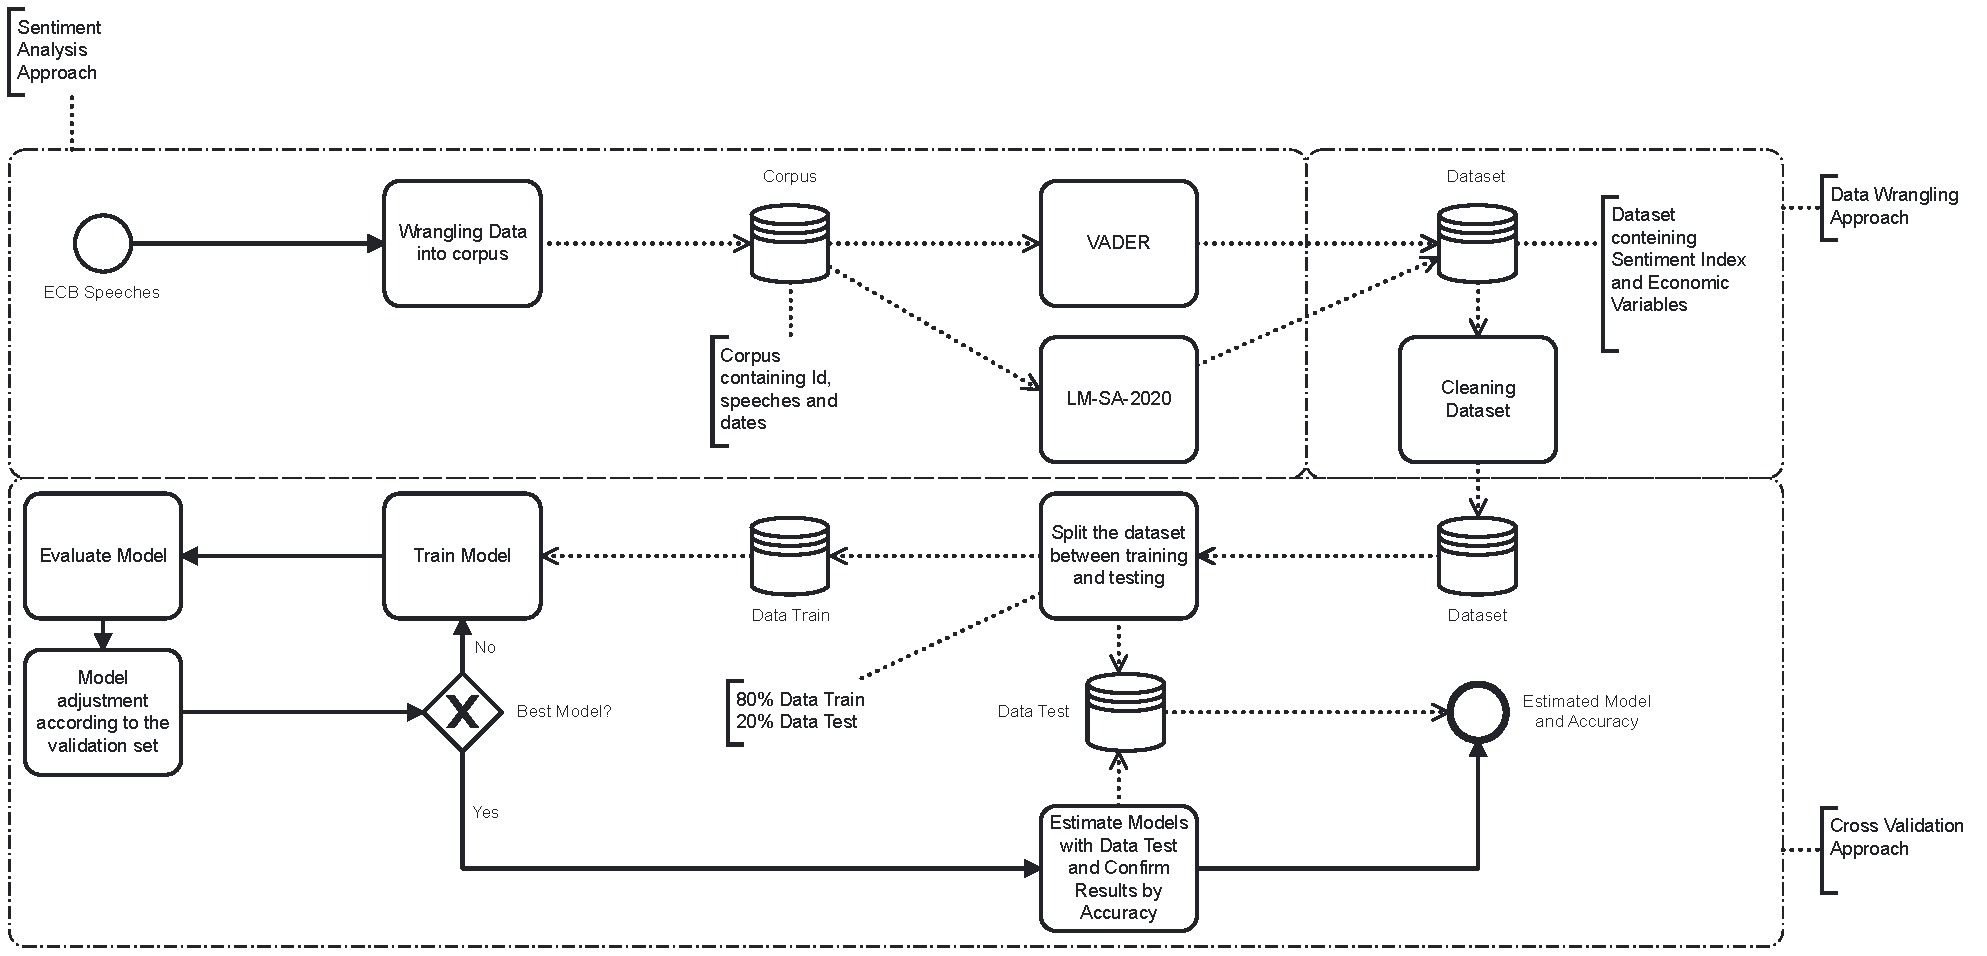
\includegraphics[width = \linewidth]{images/diagram.pdf}
    \caption*{Note: the procedure described in the flowchart defines the evolution of the project in order to describe the general procedures used. For information about the databases used, the \href{https://github.com/gustavovital/Dissertation/tree/main/data}{database repository} is free to consult}
    \label{fig:diagram}
\end{figure}
\end{landscape}


%\begin{figure}[!h]
%    \centering
%    \caption{Cross Validation Flowchart}
%    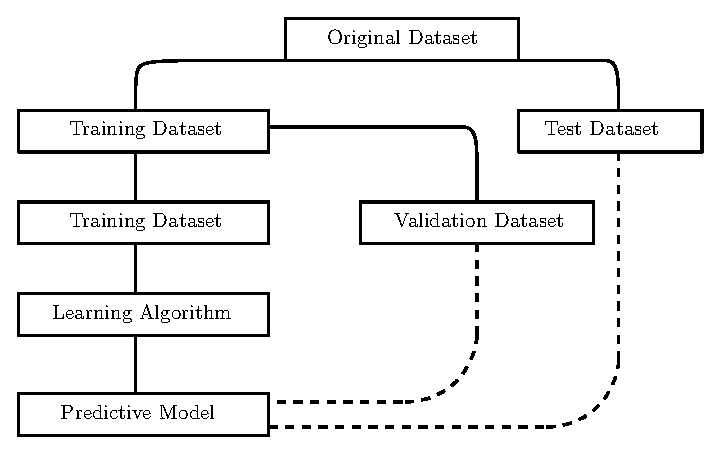
\includegraphics[width=.6\textwidth]{images/validation.eps}
%    \label{fig:cv}
%\end{figure}





%\section{Vector Autoregressive} \label{sec:var}




\newpage
\chapter{\textbf{European Central Bank Speeches: A Case Study}}

Given the need to corroborate and expand research in the area of sentiment analysis applied to the economic sciences -- and based on the examples already observed in chapter \ref{chapter:lit}, an application in a case study is proposed here.\\

% In order to add something relevant to the literature, the proposed exercises work fundamentally with observable European economic variables\footnote{it is also worth mentioning the inclusion of the output gap, obtained from the Hodrick–Prescott filter \citep{hodrick1997postwar}}: -- with the exception of the proposed sentiment index (bag of words), made from two lexicons (VADER and LM-SA)

\section{Problem and Data Description}

Following the example of \cite{shapiro2020measuring}, \cite{barsky2012information} and \cite{shapiro2020measuring}, two practical exercises are proposed.\\

Firstly, in order to understand whether a sentiment index can be used for forecasting and estimating economic variables, and following the example of \cite{shapiro2020measuring}, we propose the estimation of two LASSO models (L1 norm) in order to identify possible relevant variables in scenarios macroeconomic models -- the first model is the conventional LASSO and the second the Adaptive LASSO. Still, in order to expand the field of estimations, an elastic net model is estimated, in order to capture improvements in model specifications and improve the selection of variables when the coefficients are close to zero  when:the coefficients are close to zero, elastic net tries to take advantage of the information provided by the variables without necessarily forcing the coefficients to zero, and without considering a scenario where all variables are used in order to improve a model (L2 norm).\\

From there, the estimation of an autoregressive vector (VAR) is considered, also following the indications of the literature \citep{shapiro2020measuring, barsky2012information} to better understand how a sentiment index relates to a macroeconomic scenario (and its variables). For this, the main focus of the second exercise is the exploration of impulse and response functions obtained through VAR.

The proposed exercises work fundamentally with observable European economic variables\footnote{it is also worth mentioning the inclusion of the output gap, obtained from the Hodrick–Prescott filter \citep{hodrick1997postwar}}, with the exception of the proposed sentiment index (bag of words), made from two lexicons (VADER and LM-SA).\\

The other series used for the exercises were obtained from the website of FRED - Federal Reserve Bank of St. Louis - and they are: Consumer Price Index: Harmonized Prices: Total All Items for the Euro Area; Consumer Opinion Surveys: Consumer Prices: Future Tendency of Inflation: European Commission and National Indicators for the Euro Area\footnote{Following the guidance of \cite{shapiro2020measuring}}; Real Gross Domestic Product (Euro/ECU series) for Euro area; Long-Term Government Bond Yields: 10-year: Main (Including Benchmark) for the Euro Area; Harmonized Unemployment Rate: Total: All Persons for the Euro Area. Two dummies were also included in the exercise, the first referring to the Subprime mortgage crisis; and the second referring to the economic crisis generated by the COVID-19 pandemic.\\

%\subsection{Sentiment Indexes}

Given that both series referring to sentiment indices are also not observable, they were obtained as proxies for the speeches of the European central bank\footnote{Speeches are available at https://www.ecb.europa.eu/press/key/date/html/index.en.html}. The methodology discussed here is based on \cite{loughran2011liability}, taking into account its contribution to the literature when referring to the applicability of sentiment analysis applied to economics.\\

According to \cite[p. 35]{loughran2011liability} it is possible to measure, as well as classify an economic text from the negative words in a way that the tone of these presents a correlation with economic and financial variables, since ``The results to date indicate that negative word classifications can be effective in measuring tone, as reflected by significant correlations with other financial variables''\\

As stated by \cite[p. 13]{shapiro2021taking} ``There is a large and growing literature aimed at quantifying sentiment from text. We use a method known as the `Bag of Words' or `lexical' approach, which relies on predefined dictionaries of words that are associated with particular sentiments'' -- in this work we also consider the polarity when taking into account the VADER -- analysis from valence, given a score. Unlike VADER, where the polarity is displayed\footnote{The polarity was obtained from the Natural Language Toolkit \cite[]{bird2009natural} module for Python from positive, negative, neutral and compound words.} the polarity of each text taking into account the LM-SA-2020 and extracting the composition of negative words in order to consider the weight of each term as a function of the total terms:

\begin{quote}
``In the context of information retrieval [\dots] note that term weighting `has an enormous impact on the effectiveness of a retrieval system.' Essentially, term weighting acknowledges that raw word counts are not the
best measure of a word’s information content''\cite[p. 42]{shapiro2020measuring}  
\end{quote}
So, given the occurrence of a negative word $W_{Negative}$, its frequency is computed so that the index, based on the negative terms, is given by:
\begin{align*}
I_{Negative, i} = \frac{W_{Negative, i}}{W_{Total, i}} \quad ,
\end{align*}

Where, $I_{Negative, i}$ represents the index score given the discourse $i$ of the corpus; $W_{Negative, i}$ represents the number of negative words given the speech $i$ of the corpus; and $W_{Total, i}$ represents the total number of words (positive, negative and neutral) given the speech $i$ of the corpus. As the European central bank usually carries out more than one speech per month and the objective is the value of the monthly index, it was necessary to group the values obtained per speech around its monthly average, so that:
\begin{align*}
    I_{t} = \frac{1}{n}\sum_{i=1}^{n}I_{Negative,i} \quad
\end{align*}

That is, the monthly value of the index is given by the average of the scores of the indexes of each speech in the same month.\\

The Figure \ref{fig:correlationvaderlmsa} presents the scatter plot between the two formulated indices: VADER (valence) and LM-SA-2020 (polarity). Even though the polarity calculation methodology is different for both lexicons, the Pearson correlation coefficient between them is, as expected, positive (69.76\%).

\begin{figure}[!h]
    \centering
    \caption{Correlation between the polarities obtained from the VADER and LM-SA-2020 lexicons (negative words)}
    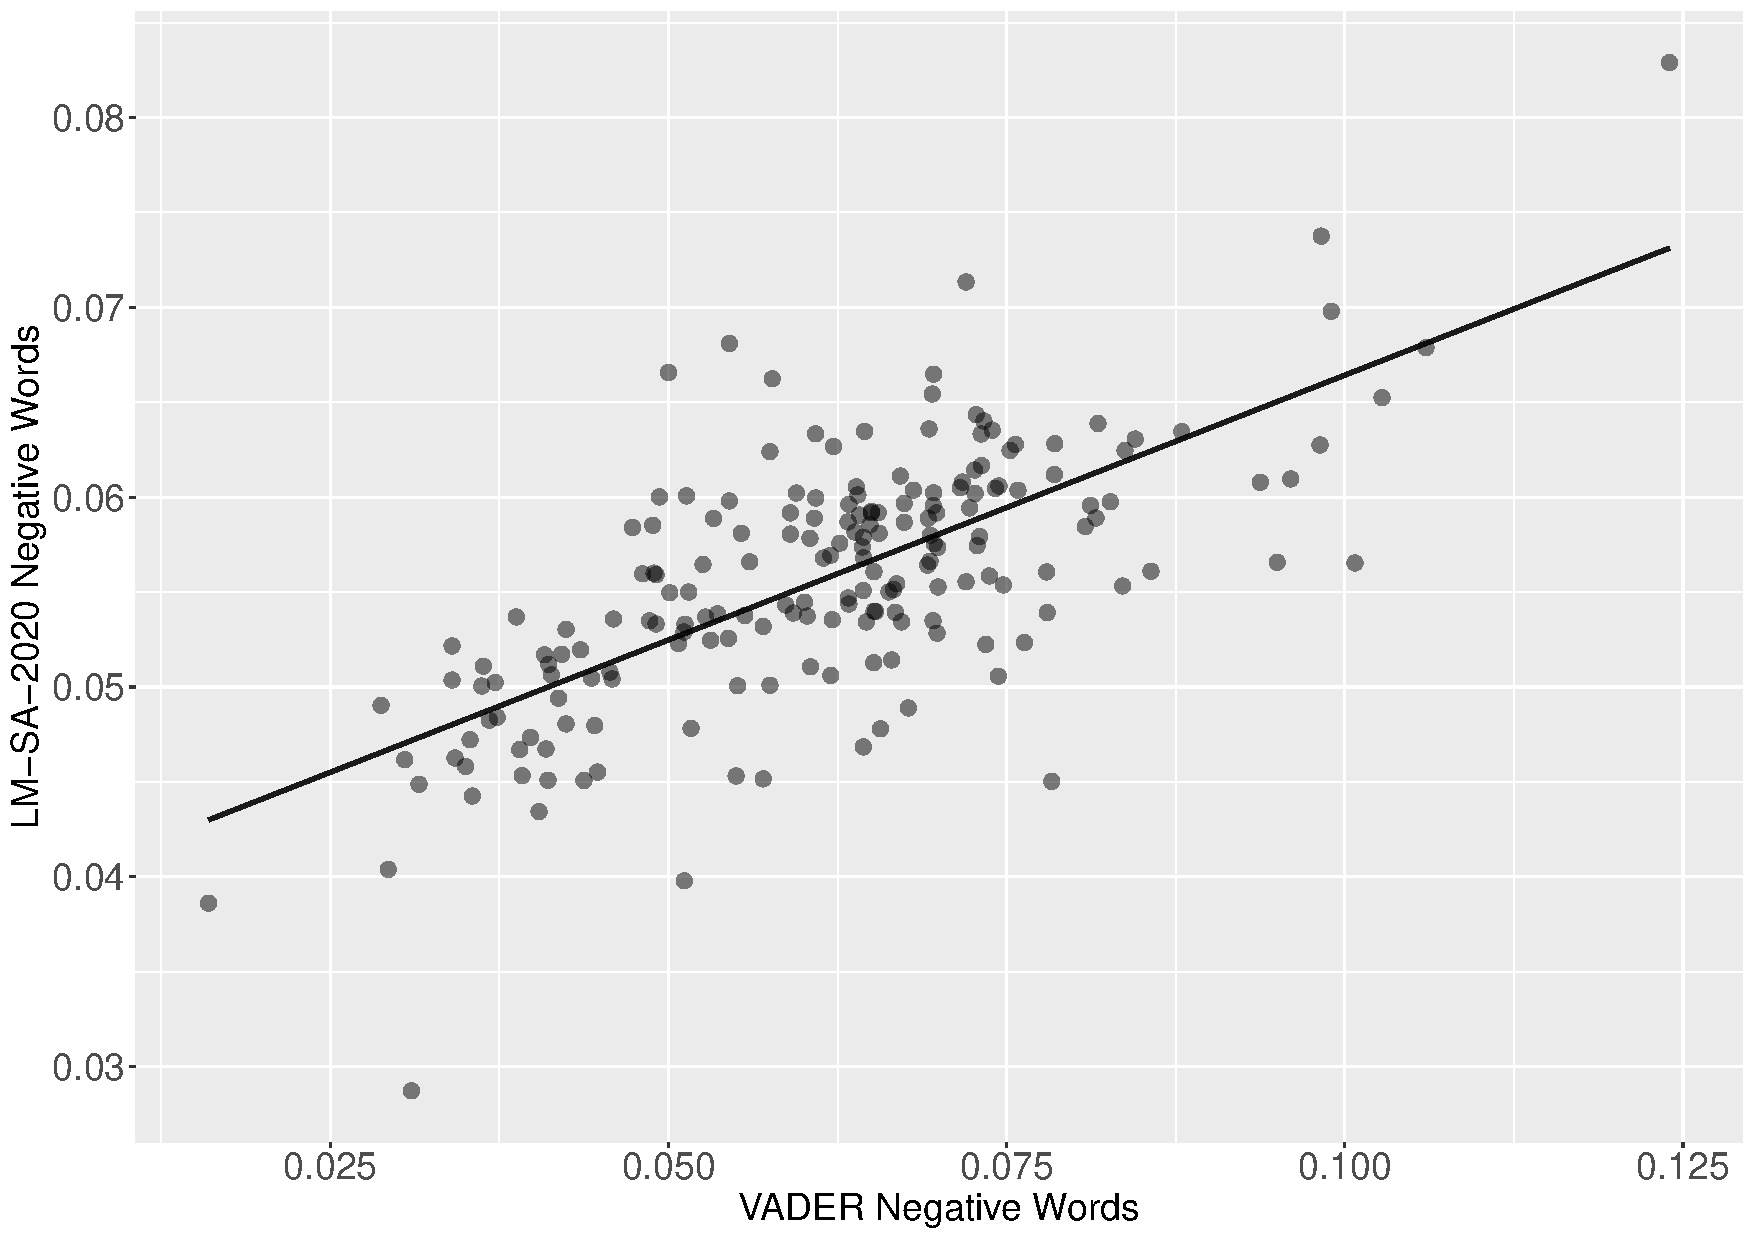
\includegraphics[width=.7\textwidth]{images/correlation_vader_lm.pdf}
    \label{fig:correlationvaderlmsa}
\end{figure}

Both indices are used in the case studies. At first, it would be recommended to \cite[p. 62]{loughran2011liability} the main use of a lexicon focused on economic and financial terms and words (LM-SA-2020) -- however, VADER is used due to the excellent results that this lexicon presents. Furthermore, it is considered an exercise to compare both lexicons: in consideration of the fact that the LM-SA-2020 focuses on economic and financial terms and words, in contrast to VADER, which, even being aimed at media analysis, has excellent results against similar lexicons.

\section{Experimental Setup}

Since the case studies consider certain statistical and econometric techniques, it is necessary to consider some assumptions in relation to the methodologies adopted and to analyze the behavior of the time series.\\

The time horizon adopted was from January 2005 to December 2020 -- it was not possible to extend this work until the year 2021 due to lack of data at the time of writing this: moreover, the choice of period was arbitrary, considering , however, the availability of the economic series and the availability of the speeches of the European Central Bank used. In all, the original database is composed of 132 observations so that two of the variables are sentiment indices (VADER and LM-SA-2020); two dummies are considered for the estimation of the variable selection models, namely: 1st- COVID, so that if the time point is February, March, or April 2020, COVID = 1, otherwise COVID = 0; 2nd - Debt Crisis in Europe, so that if the time period is from September 2011 to January 2013, the dummy assumes the value of 1, otherwise 0; all other variables are observable economic variables -- with the exception of the output gap, obtained from the Hodrick-Prescott filter.\\

In addition, it is noteworthy that, for convenience in relation to the estimations and the number of observations, it was chosen to use series of monthly frequency.\\

Also regarding the behavior of the series, two unit root tests were performed to verify the stationarity condition: the Augmented-Dickey-Fuller \cite[]{cheung1995lag} and the Phillips \& Perron Unit Root Test \cite[]{phillips1988testing} -- both were estimated from the URCA package \cite[]{urcacran} from the R software \cite[]{rcran}. Since in one of the case studies the stationarity condition is necessary for the exercise to be carried out, the series that are not zero-order I(0) integrated must be treated.\\

Basically, the Augmented-Dickey-Fuller and Phillips \& Perron tests consist of verifying whether the time series have a unit root. In the case of the Augmented-Dickey-Fuller test, given the equation:
\begin{align}
    \Delta y_t = \alpha + \beta t + \gamma y_{t-1} + \sum_{i=1}^{p} \delta_i \Delta y_{t-i} + \varepsilon_t
\end{align}
where $\alpha$ is the model constant, $\beta$ the coefficient related to the trend, $p$ is the order of the autoregressive process and $\Delta$ represents the difference in the series. If both $\alpha$ and $\beta$ are not significant for the model, that is $\alpha = 0$ and $\beta = 0$, the variation of $y$ in $t$ will be explained only by $\varepsilon$, that is, by a white noise.\\

The Phillips \& Perron unit root test, in turn, considers a model with an autoregressive process of order 1, so that:
\begin{align}
    y_t = \alpha + \beta t + \phi y_{t-1} + \varepsilon_t
\end{align}
where $\alpha$ is the model constant, $\beta$ the coefficient related to the trend, $\phi$ is the coefficient related to a first order autoregressive process and $\varepsilon$ is a white noise. Again, if $\alpha=0$ and $\beta = 0$ we are dealing with a situation where the series $y_t$ is explained only by a white noise, thus characterizing a random walk -- that is: the series is non-stationary. \\

Both tests were performed for all series, with the exception of the indices of sentiments in difference, since both indices were stationary at level, these were only tested for level. In relation to the other variables tested (Table {\ref{tab:urlevel}}), only the Product Gap (statistically significant at 1\% with trend ADF test); Producer Prices Index (statistically significant at 5\% PP test) and Interest Rate (statistically significant
at 10\% ADF) were identified as stationary. 


\begin{table}[!h]
\caption{Unit Root Tests: Augmented-Dickey-Fuller and Phillips \& Perron}
\begin{adjustbox}{max width=\textwidth}
\begin{tabular}{lllllllllll} 
\hline
                               & \multicolumn{6}{c|}{Augmented-Dickey-Fuller}                                        & \multicolumn{4}{c}{Phillips \& Perron}                    \\ \cline{2-11} 
                               & \multicolumn{2}{c|}{None} & \multicolumn{2}{c|}{Drift} & \multicolumn{2}{c|}{Trend} & \multicolumn{2}{c|}{Constant} & \multicolumn{2}{c}{Trend} \\ \hline
Consumer Opinion Surveys       & -0.69189        &         & -2.46604        &          & -2.57411        &          & -2.51257          &           & -2.59686        &         \\
Unemployment Rate              & -1.12625        &         & -0.16789        &          & -1.60657        &          & -0.12221          &           & -1.71892        &         \\
Interest Rate                  & -1.90764        & *       & -0.99368        &          & -2.52323        &          & -0.95965          &           & -2.54834        &         \\
Consumer Price Index           & -0.9864         &         & -1.16925        &          & -1.96056        &          & -1.23476          &           & -1.958          &         \\
Gap Gross Domestic Product     & 0.576651        &         & -2.03914        &          & -4.33739        & *        & -1.6031           &           & -2.97149        &         \\
Producer Prices Index          & 0.726163        &         & -3.11724        & *        & -2.92142        &          & -2.99263          & *         & -2.64357        &         \\
Negative Sentiment (VADER)     & -1.15748        &         & -7.23406        & *        & -8.13027        & *        & -9.89749          & *         & -10.5938        & *       \\
Negative Sentiment LM-SA-2020) & -0.57929        &         & -7.39231        & *        & -7.36532        & *        & -9.93006          & *         & -9.89294        & *       \\ \hline
\end{tabular}
\end{adjustbox}
\caption*{Note: * symbolizes that the series do not reject the null hypotheses of the tests, in the absence of a unit root. The test statistics, for the Augmented-Dickey-Fuller test for none, drift and trend are respectively for 10\%, 5\% and 1\%:-2.58, -1.95, -1.62; -3.46, -2.88, -2.57; -3.99, -3.43 and -3.13. For Phillips \& Perron test for constant and trend are respectively for 10\%, 5\% and 1\%: -3.48, -2.88, -2.58; -4.03, -3.44 and -3.15.}
\label{tab:urlevel}

\end{table}

In order to follow the economic literature, and with the exception of the Product Gap variable, the series are treated as difference and, thus, the unit root tests are redone\footnote{The sentiment indices and Product Gap are, therefore, , worked at level}.\\

\section{Pre-Processing Data}
In order to treat the variables in order to obtain the stationarity condition, we now proceed to treat the series in difference, since the series that are not stationary are first-order I(1) integrated, we work with the series from the first difference.\\

When running the tests in difference all series, both tests reject the null hypothesis of unit root at 1\% (Table \ref{tab:urdiff}). The need to verify the stationarity condition becomes essential for one of the proposed case studies: the estimation of an Vector Autoregressive is not possible if any of the variables does not fulfill this condition.


% --------------------------------------------------

\begin{table}[!h]
\caption{Unit Root Tests for the Series in Difference: Augmented-Dickey-Fuller and Phillips \& Perron}
\begin{adjustbox}{max width=\textwidth}
\begin{tabular}{lllllllllll}
\hline
                           & \multicolumn{6}{c|}{Augmented-Dickey-Fuller}                                        & \multicolumn{4}{c}{Phillips \& Perron}                    \\
                           & \multicolumn{2}{c|}{None} & \multicolumn{2}{c|}{Drift} & \multicolumn{2}{c|}{Trend} & \multicolumn{2}{c|}{constant} & \multicolumn{2}{c}{trend} \\ \hline
Consumer Opinion Surveys   & -7.38867        & *       & -7.36197        & *        & -7.37293        & *        & -9.22024          & *         & -9.2483         & *       \\
Unemployment Rate          & -4.59511        & *       & -4.65701        & *        & -4.78258        & *        & -7.60278          & *         & -7.70628        & *       \\
Interest Rate              & -7.35245        & *       & -7.56178        & *        & -7.53145        & *        & -9.97176          & *         & -9.9337         & *       \\
Consumer Price Index       & -7.03739        & *       & -7.04257        & *        & -7.03008        & *        & -11.1771          & *         & -11.2587        & *       \\
Gap Gross Domestic Product & -6.87391        & *       & -6.9118         & *        & -6.89305        & *        & -6.57819          & *         & -6.55389        & *       \\
Producer Prices Index      & -6.07706        & *       & -6.11674        & *        & -6.21462        & *        & -6.08898          & *         & -6.19294        & *       \\ \hline
\end{tabular}
\end{adjustbox}
\caption*{Note: * symbolizes that the series do not reject the null hypotheses of the tests, in the absence of a unit root. The test statistics, for the Augmented-Dickey-Fuller test for none, drift and trend are respectively for 10\%, 5\% and 1\%:-2.58, -1.95, -1.62; -3.46, -2.88, -2.57; -3.99, -3.43 and -3.13. For Phillips \& Perron test for constant and trend are respectively for 10\%, 5\% and 1\%: -3.48, -2.88, -2.58; -4.03, -3.44 and -3.15.}
\label{tab:urdiff}
\end{table}

Given that the series are stationary in difference, for the VAR case study, we will use them like this, for the other exercise the series will remain level.

\section{Modeling}

Two exercises are proposed, as previously mentioned. First, a case study will be carried out taking into account the inclusion of sentiment indices when considering economic models when utilizing Variable Selection Models criteria. For this, the LASSO, Adaptive LASSO and Elastic Net models are used.\\

The second case study refers to an Autoregressive Vector (VAR) -- impulse response functions are used to better understand the behavior of macroeconomic variables when a shock is given to one of the sentiment indices (VADER and LM- SA-2020).\\

\subsection{Variable Selection Models}

Variable selection models have as main objective the identification and statistically significant variables for a model. Unlike information criteria such as AIC \cite[]{akaike1974new} and BIC \cite[]{schwarz1978estimating}, the variable selection models used here are variations of the conventional LASSO model. That is, the selection of variables is done by forcing the coefficients related to each variable to 0 when not significant, so that when significant, the coefficients are greater than 0.\\

The first method of Variable Selection Models used in this first case study is the conventional LASSO. The LASSO estimator (least absolute shrinkage and selection operator) is a linear estimation method presented in 1996 in a paper entitled ``Regression Shrinkage and Selection via the lasso'' \cite[]{tibshirani1996regression}. For regressions and generalized regressions, this estimator was proposed as a shrinkage and selection method.\\

Assuming a data set such that $(x^i, y_i)$ and $i = 1, 2, \dots , N$, and assuming $x^i = (x_{i1}, \dots, x_{ip})^T$ are the predictor variables and $y_i$ is the dependent variable. Also, since $\hat{\beta} = (\beta_1, \dots, \beta_p)^T$ the estimate LASSO $(\hat{\beta}^{lasso})$ \cite[p. 268]{tibshirani1996regression} is given in its Lagrangian equivalent by:

\begin{align} \label{eq:lasso}
    \hat{\beta}^{lasso} = \frac{1}{2}(y - Xb)'(y - Xb) + \lambda\sum_{j=1}^p|b_j|
\end{align}
the penalty on $\sum_1 ^p |\beta_j|$ is called the L1 lasso penalty \cite[p.68]{hastie2009elements} and this last constraint makes the solution nonlinear in $y_i$. The LASSO, however, ``does not focus on subsets but rather defines a continuous shrinking operation that can produce coefficients that are exactly 0''\cite[p.286]{tibshirani1996regression}. Thus, it can be seen that the greater $\lambda$, the greater the number of coefficients defined as 0. The value of $\lambda$ in this case study is obtained by cross validation following the literature\cite[p. 136]{hoornweg2018science}.\\

Another estimator used in this case study as a variable selection model is the first variation of the LASSO presented here. The  Adaptive lasso estimator was first described by \cite{zou2006adaptive} and, in contrast to lasso, augments the penalty with a vector of weights. The adaptive LASSO estimator ($\hat{\beta}^{alasso}$), then, is given by:

\begin{align} \label{eq:lassoadaptive}
    \hat{\beta}^{alasso} = \frac{1}{2}(y - Xb)'(y - Xb) + \lambda\sum_{j=1}^p\hat{w}_j |b_j|
\end{align}

Where $\hat{w}_j$ is a vector of weights and can ``be given by $\hat{w}_j = \frac{1}{|b_{ols, j}|^\gamma}$, for some $ \gamma > 0$'' \cite[p. 115]{hoornweg2018science}.\\

The third variable selection model used here is the Elastic Net model \cite[]{zou2005regularization}. Despite the fact that there are more choices for other LASSO models, like the random LASSO \cite[]{wang2011random} and the group LASSO \cite[]{yuan2006model}, Elastic Net was used for being a well-known reference in the literature and for combining the L2 penalty\footnote{The L2 penalty is also known as Ridge regression \cite[p.2]{owen2007robust}.}:

\begin{align}\label{eq:elasticnet}
    \hat{\beta}^{enet} = \frac{1}{2}(y - Xb)'(y - Xb) + \lambda\sum_{j=1}^p\left(\frac{\alpha}{2}b_j ^2 + (1 - \alpha)|b_j|\right)
\end{align}
The formulation presented in (\ref{eq:elasticnet}) is the same formulation presented by \cite{hastie2009elements}. The Elastic Net model introduces a parameter $\alpha$ into the model so that when $\alpha = 0$ the model only incorporates the L1 LASSO penalty; and when $\alpha = 1$ the model only incorporates the L2 Ridge penalty; when $0 < \alpha < 1$ the Elastic Net model incorporates properties from both the LASSO model and the Ridge model. In this case, both $\lambda$ and $\alpha$ were obtained from cross validation.


\subsection{Vector Autoregression}

In order to consider a deeper analysis in terms of economic simulation, and taking into account the endogeneity characteristic, a Vector Autogression (VAR) model is estimated as a second case study. In mathematical terms, we can represent a VAR(1) in a matrix form, that is, a first-order Autoregressive Vector as follows:

\begin{align} \label{eq:var1}
    \begin{bmatrix}
    y_{1,t} \\
    y_{2,t}
    \end{bmatrix} = 
    \begin{bmatrix}
    \delta_1\\
    \delta_2
    \end{bmatrix} +
    \begin{bmatrix}
    \phi_{11} & \phi_{12} \\
    \phi_{21} & \phi_{22}
    \end{bmatrix}
    \begin{bmatrix}
    y_{1,t-1} \\
    y_{2,t-1}
    \end{bmatrix} +
    \begin{bmatrix}
    \varepsilon_{1,t} \\
    \varepsilon_{2,t}
    \end{bmatrix} 
\end{align}

Where $y_1$ and $y_2$ are endogenous variables and $\varepsilon_1$ and $\varepsilon_2$ are the error terms for each equation. $\phi_{12}$ represents, in turn, the linear dependence of $Y_{1, t}$ on $y_{2, t-1}$ given the presence of $y_{1, t-1}$ . Thus, if $\phi_{12} = 0$, then $y_{1, t}$ does not depend on $y_{2, t-1}$ when $y_{2, t-1}$ is given. \\

Also, according to \cite{verbeek2008guide}, we can represent a first-order Autoregressive Vector as follows:

\begin{align*}
    \overrightarrow{Y_t} = \phi + \theta \overrightarrow{Y_{t-1}} + \overrightarrow{\varepsilon_t} \quad ,
\end{align*}
where, for a VAR(1) with two variables: $\overrightarrow{Y_t} = [y_{1,t}, y_{2, t}]'$ and $\overrightarrow{\varepsilon_t} = [\varepsilon_{1, t}, \varepsilon_{2, t}]$. Thus, in general a VAR(P) can be written as follows:

\begin{align*}
    \overrightarrow{Y_t} = \phi + \theta_1 \overrightarrow{Y_{t-1}} + \dots + \theta_p \overrightarrow{Y_{t-p}} + \overrightarrow{\varepsilon_t} \quad ,
\end{align*}
where each $\theta_j$ is a matrix $k \times k$ and $\overrightarrow{\varepsilon_t}$ is a vector of length $k$ of white noises, with a covariance matrix defined by $\sum$.\\

For each of its parts, the VAR model implies an ARMA model. Since the information set is expanded to additionally include the history of other variables, evaluating the components simultaneously has the advantages of being more parsimonious, containing fewer lags, and allowing for more accurate predictions \cite[p.322]{verbeek2008guide}. From a different angle, \cite{sims1980macroeconomics} asserts that using VAR models rather than simultaneous structural equations is advantageous since no 'arbitrary' limitations or previous assumptions need to be made regarding the separation between exogenous and endogenous variables.\\

In the same way that we can represent an Autoregressive from its moving average component, we can also write a VAR as a moving average vector. Considering the equation (\ref{eq:var1}, we can represent it as follows:

\begin{align} \label{eq:mavar1}
    \begin{bmatrix}
    y_{1,t} \\
    y_{2,t}
    \end{bmatrix} = 
    \begin{bmatrix}
    \bar{y_1}\\
    \bar{y_2}
    \end{bmatrix} + \sum_{i=0}^{\infty}
    \begin{bmatrix}
    \phi_{11} & \phi_{12} \\
    \phi_{21} & \phi_{22}
    \end{bmatrix}^i
    \begin{bmatrix}
    \varepsilon_{1,t-i} \\
    \varepsilon_{2,t-i}
    \end{bmatrix} 
\end{align}
Where $y_{1, t}$ and $y_{2, t}$ are expressed in terms of \{$\varepsilon_{1, t}$\} and \{$\varepsilon_{1, t}$\} respectively. According to \cite{enders2008applied}, it is possible to rewrite the previous equation in terms of \{$\varepsilon_{y1, t}$\} and \{$\varepsilon_{y2, t}$\}. Thus, the error vector can be written as follows:

\begin{align} \label{eq:varvarepsilon}
    \begin{bmatrix}
    \varepsilon_{1,t} \\
    \varepsilon_{1,t}
    \end{bmatrix} = \frac{1}{1 - b_{12}b_{21}}
    \begin{bmatrix}
    1 & -b_{12} \\
    -b_{21} & 1
    \end{bmatrix}
    \begin{bmatrix}
    \varepsilon_{y1, t} \\
    \varepsilon_{y2, t}
    \end{bmatrix}
\end{align}
combining the equations (\ref{eq:mavar1}) and (\ref{eq:varvarepsilon}), we obtain:

\begin{align*}
    \begin{bmatrix}
    y_{1,t} \\
    y_{2,t}
    \end{bmatrix} =
    \begin{bmatrix}
    \bar{y_1}\\
    \bar{y_2}
    \end{bmatrix} + \frac{1}{1 - b_{12}b_{21}} \sum_{i=0}^{\infty}
    \begin{bmatrix}
    \phi_{11} & \phi_{12} \\
    \phi_{21} & \phi_{22}
    \end{bmatrix}^i
    \begin{bmatrix}
    1 & -b_{12} \\
    -b_{21} & 1
    \end{bmatrix}
    \begin{bmatrix}
    \varepsilon_{y1, t} \\
    \varepsilon_{y2, t}
    \end{bmatrix} \quad ,
\end{align*}
replacing the matrix $2 \times 2$ with a generic term to simplify the notation:

\begin{align}
    \Gamma_i = \frac{A_1 ^i}{1 - b_{12}b_{21}}\begin{bmatrix}
    1 & -b_{12}\\
    -b_{21} & 1
    \end{bmatrix}
\end{align}
therefore, the moving media representation presented in (\ref{eq:mavar1}) and (\ref{eq:varvarepsilon}) can be expressed as:

\begin{align} \label{eq:mavar1}
    \begin{bmatrix}
    y_{1,t} \\
    y_{2,t}
    \end{bmatrix} = 
    \begin{bmatrix}
    \bar{y_1}\\
    \bar{y_2}
    \end{bmatrix} + \sum_{i=0}^{\infty}
    \begin{bmatrix}
    \Gamma_{11}(i) & \Gamma_{12}(i) \\
    \Gamma_{21}(i) & \Gamma_{22}(i)
    \end{bmatrix}^i
    \begin{bmatrix}
    \varepsilon_{y1, t} \\
    \varepsilon_{y2, t}
    \end{bmatrix} \quad ,
\end{align}
or in a more compact form:

\begin{align*}
    x_t = \epsilon + \sum_{i=0}^{\infty}\Gamma_i \varepsilon_{t-1}
\end{align*}
In terms of analysis, the final equation offers a very helpful tool to look at how the variables $y_1$ and $y_2$ interact with one another. For time periods of $y_1$ and $y_2$, the effects of $\varepsilon_{y1, t}$ on shocks of $\varepsilon_{y1, t}$ can be generated using the coefficients of $\Gamma_i$. As a result, it is clear that the four components of $\Gamma_{jk}(0)$ are effect multipliers \cite[p.295]{enders2008applied}.\\

By correctly adding the coefficients of the \textit{impulse response functions}, it is possible to determine the overall effects of an impulse on $\varepsilon_{y1, t}$ and/or $\varepsilon_{y2, t}$. For instance, we can observe that the impact of $\varepsilon_{y2, t}$ on the value of $y_{1+n}$ after $n$ periods is $\Gamma_{12}(n)$. The cumulative sum of $\varepsilon_{y2, t}$ effects on $y_1$ after n periods is as follows:

\begin{align*}
    \sum_{i=0}^{n}\Gamma_{12}(i) \quad ,
\end{align*}
if $y_1$ and $y_2$ are stationary, the values of $\Gamma_{jk}(i)$ converge to zero, the larger $i$ is. Shocks cannot, therefore, permanently alter stationary series. Thus, it follows:

\begin{align*}
    \sum_{i=0}^{\infty}\Gamma^2 _{jk}(i) \text{ is finite,}
\end{align*}
the four sets of coefficients $\Gamma_{11}(i)$, $\Gamma_{12}(i)$, $\Gamma_{21}(i)$ and $\Gamma_{22}(i)$ are called the impulse response function.

\section{Cross Validation and Learning Algorithms}

Cross Validation is a technique widely described in the literature \cite[]{hoornweg2018science, hastie2009elements, stone1974cross, breiman1992submodel} that aims to obtain optimal parameters from a predefined model. In Cross Validation, the dataset is divided between a training dataset and a test dataset, these being composed of 80\% and 20\% of the original dataset \cite[291]{breiman1992submodel}. The model, then, ``is estimated with a training sample and these estimates are used to ‘predict’ the outcomes of the validation sample. By varying the choice of a tuning parameters, one can select the set of configurations that leads to the best pseudo-out-of-sample forecasts''\cite[p.136]{hoornweg2018science}.\\

\begin{figure}[!h]
    \centering
    \caption{Cross Validation Flowchart}
    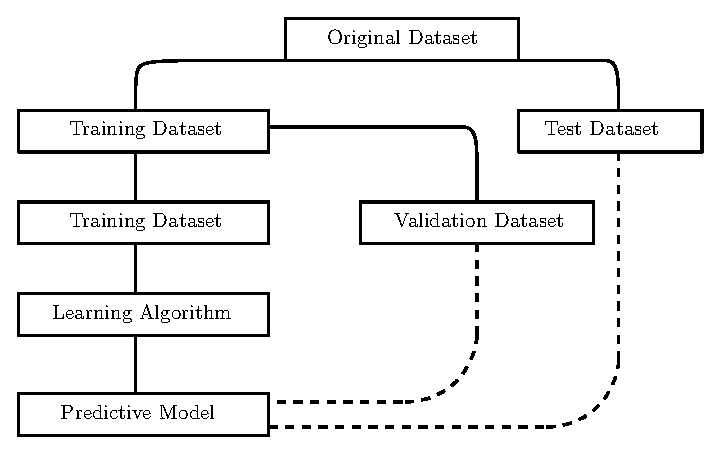
\includegraphics[width=.6\textwidth]{images/validation.eps}
    \label{fig:cv}
\end{figure}


Figure \ref{fig:cv} presents a flowchart explaining how Cross Validation works. The same procedure was performed for the models estimated in this work (LASSO, Adaptive LASSO, and Elastic Net). Both the training, validation, and test dataset division were done randomly using the texttt{Matrix} \cite[]{matrix2020cran} package of the R software.\\

Four evaluation metrics criteria were taken into consideration when performing the cross validation procedure for the variable selection models. The $R^2$ \cite{heinisch1962steel}, the MAE \cite{willmott2005advantages}, the MSE \cite{bickel2015mathematical}, and the RMSE \cite{hyndman2006another}. Based on these criteria, the values of $\lambda$ were selected for the LASSO and Adaptive LASSO models, and the values of $\lambda$ and $\alpha$ for the Elastic Net model. For the VAR models, in addition to the AIC and BIC selection criteria, the Hannan–Quinn information criterion \cite{hannan1979determination} was also used.\\

From there, the selected models were analyzed and the results will be presented in the next  section  \ref{sec:expresults}.

\section{Experimental Results} \label{sec:expresults}


\begin{figure}[!h]
    \centering
    \caption{Impulse Response of a Sentiment Index (LM-SA) Shock on Economic Activity}
    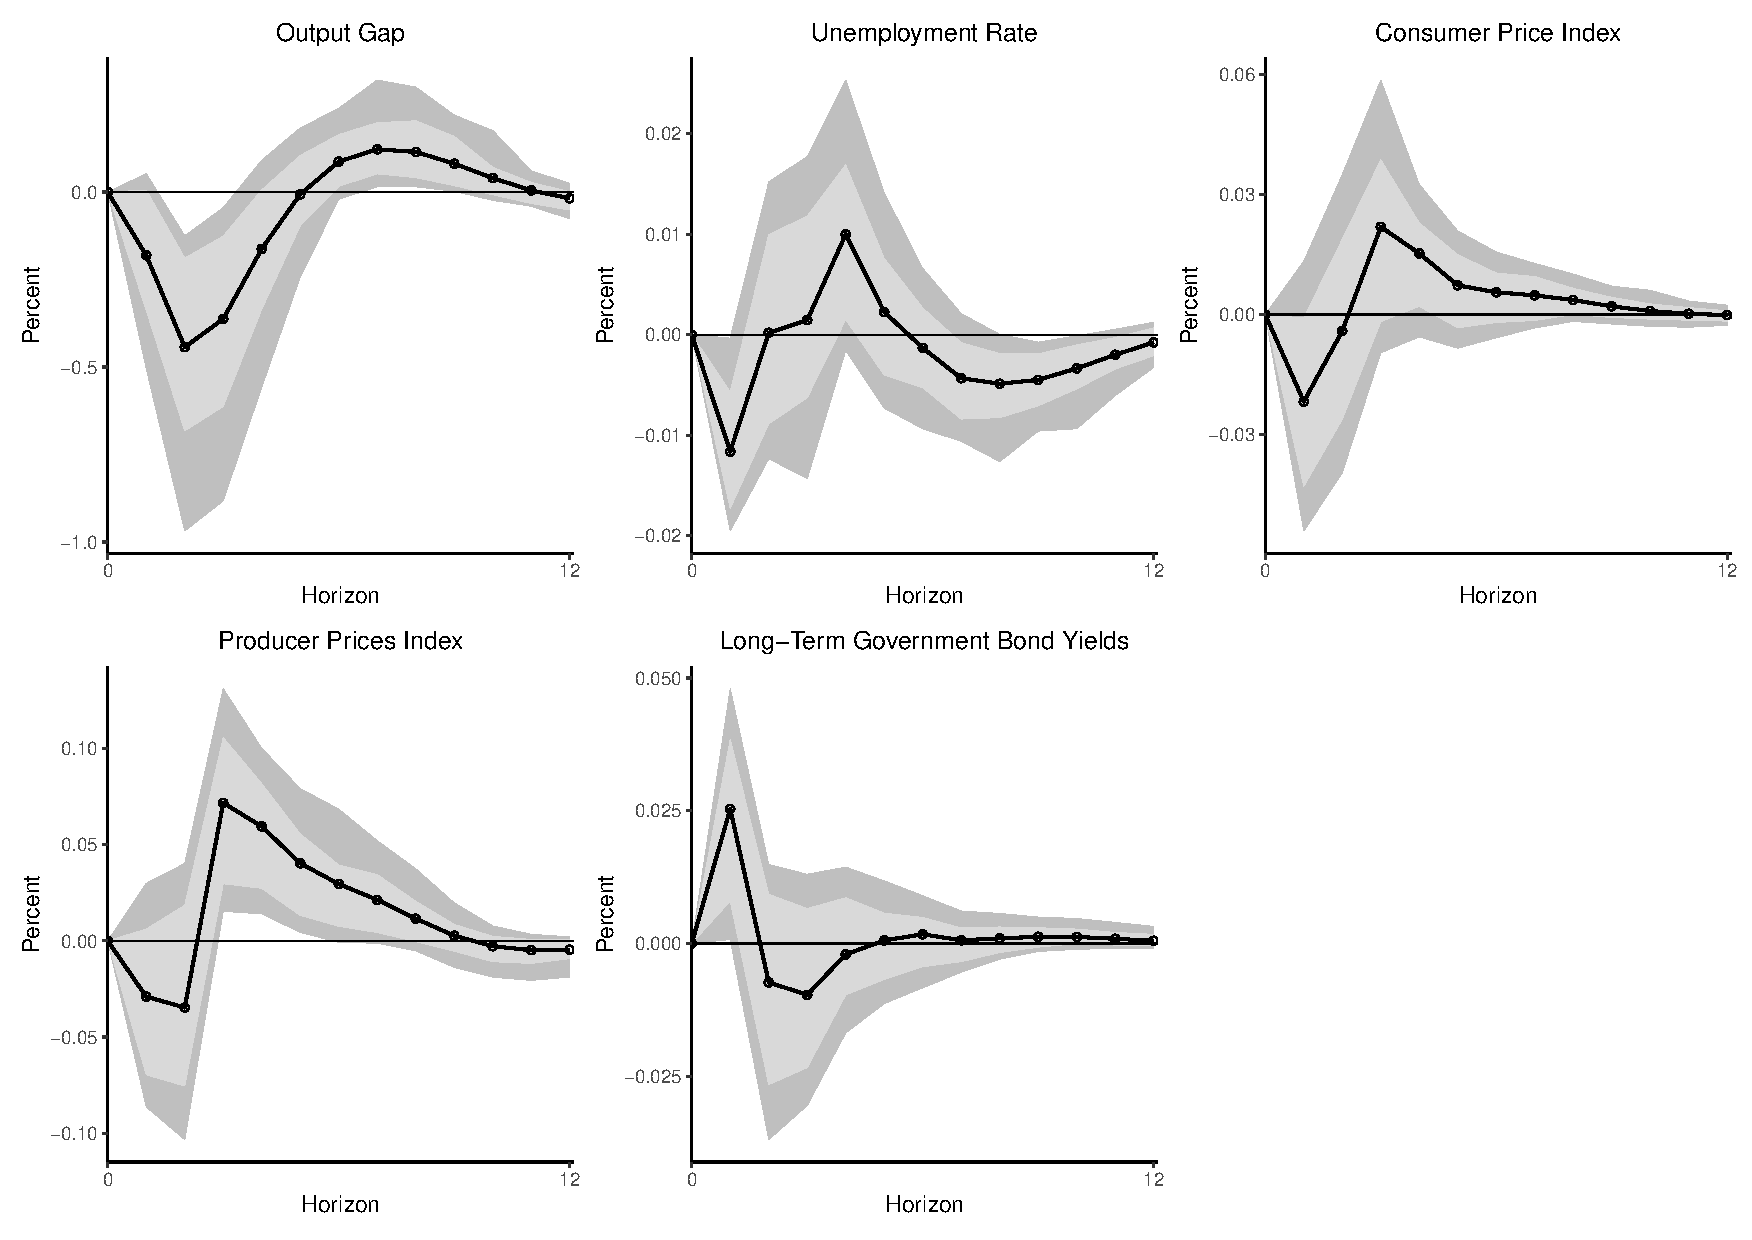
\includegraphics[width=\textwidth]{images/irf_lm.pdf}
    \caption*{Impulse Response from a sentiment index shock (LM-SA). The variables are described as follows: Output gap -- obtained from a HP filter from Real Gross Domestic Product (Euro/ECU series) for Euro area; Unemployment Rate -- Harmonized Unemployment Rate: Total: All Persons for the Euro Area}
    \label{fig:irflm}
\end{figure}


\begin{figure}
    \centering
    \caption{Impulse Response of a Sentiment Index (VADER) Shock on Economic Activity}
    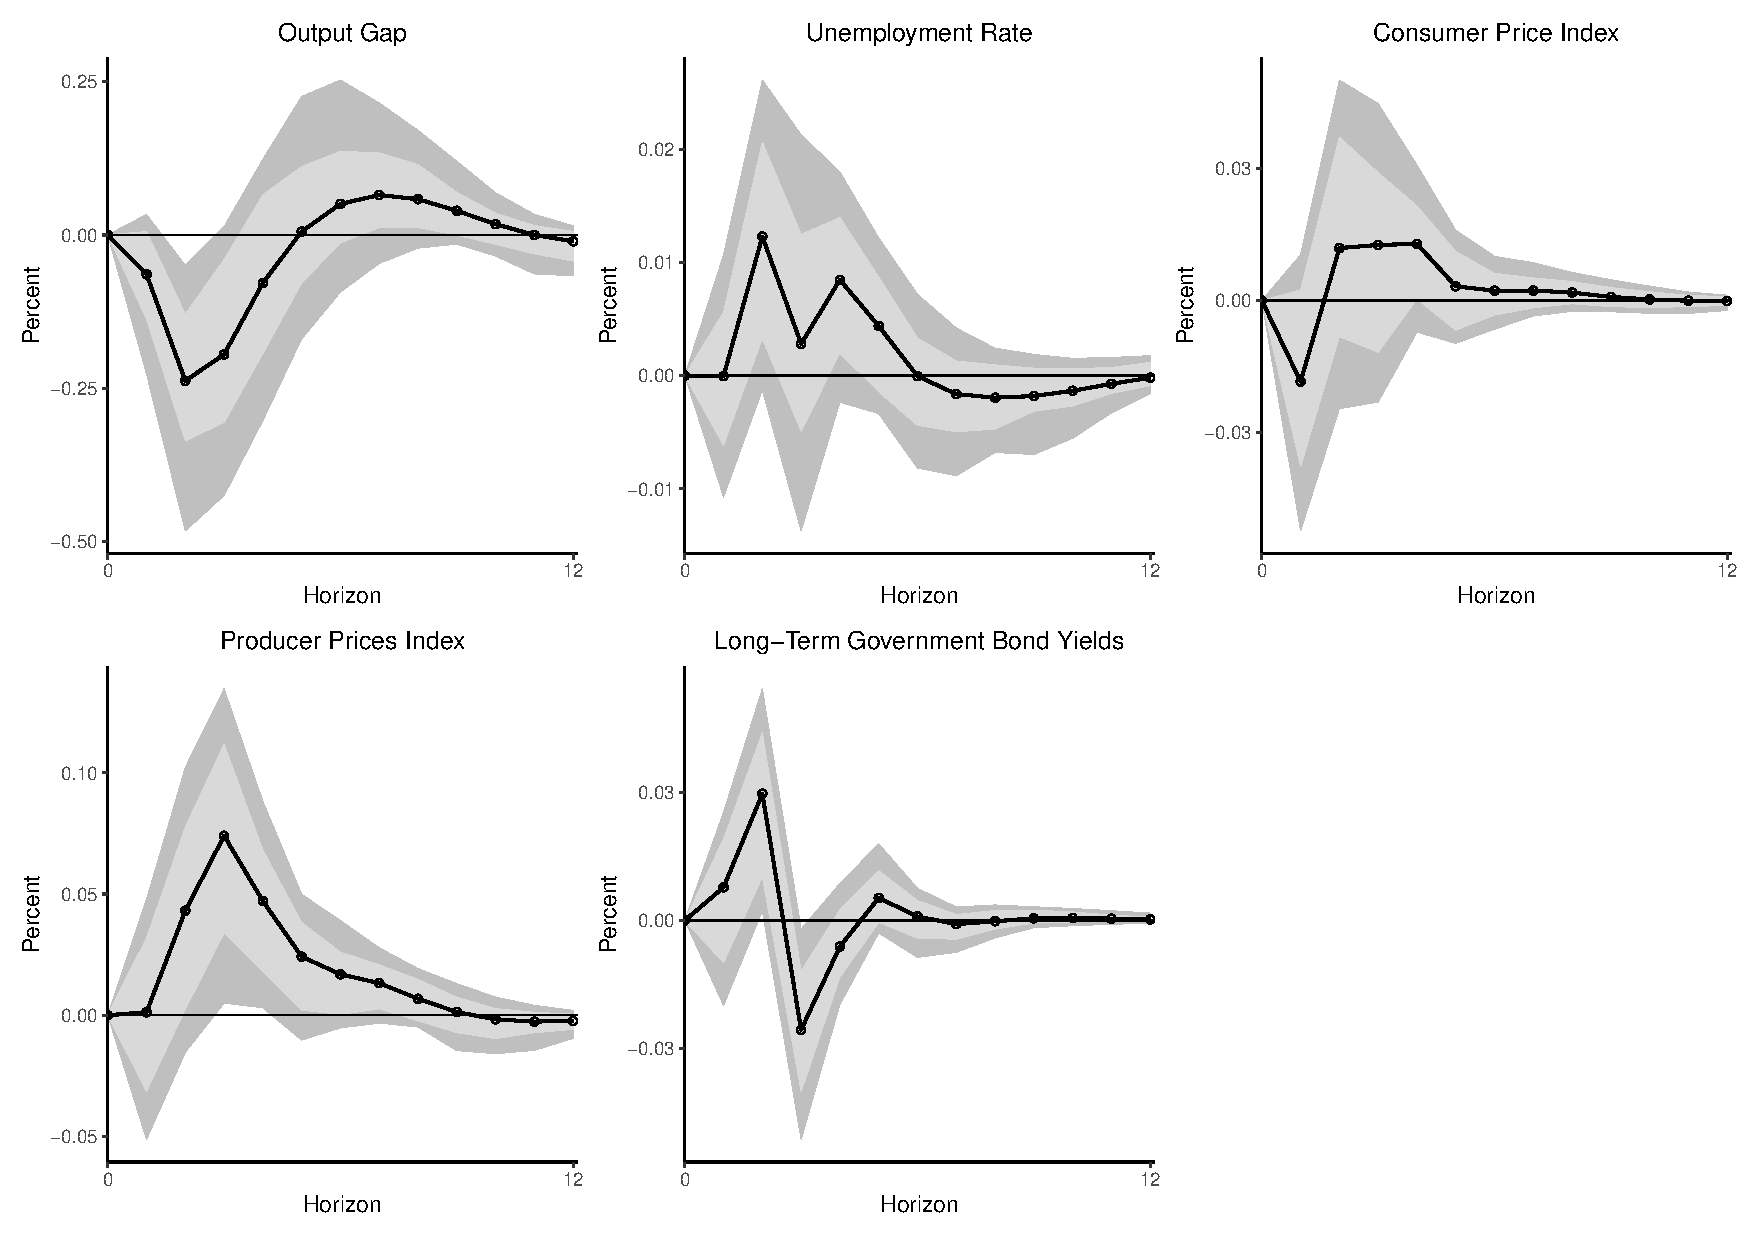
\includegraphics[width=\textwidth]{images/irf_vader.pdf}
    \caption{Caption}
    \label{fig:my_label}
\end{figure}

\section{Discussion}

\begin{landscape}


\begin{table}[]
\caption{Variable Selection Models: VADER Sentiment}
\label{tab:selectionvader}
\begin{adjustbox}{max width=\linewidth}
\begin{tabular}{llllllllll}
\hline
                         & \multicolumn{3}{c}{Consumer Opinion   Surveys} & \multicolumn{3}{c}{Unemployment Rate}      & \multicolumn{3}{c}{Interest Rate}         \\
                         & Lasso     & Adaptive Lasso    & Elastic Net    & Lasso    & Adaptive Lasso   & Elastic Net  & Lasso   & Adaptive Lasso   & Elastic Net  \\
Consumer Opinion Surveys & x         &                   & x              & x        &                  & x            & x       & x                & x            \\
Unemployment Rate        & x         & x                 & x              & x        & x                & x            & x       & x                & x            \\
Interest Rate            & x         & x                 & x              &          &                  & x            & x       & x                & x            \\
Consumer Price Index     & x         & x                 & x              & x        & x                & x            & x       & x                & x            \\
Gross Domestic Product   & x         &                   & x              &          & x                & x            & x       & x                & x            \\
Producer Prices Index    & x         & x                 & x              & x        & x                & x            & x       & x                & x            \\ \hline
VADER Sentiment          & x         & x                 & x              &          & x                & x            & x       & x                & x            \\ \hline
                         & \multicolumn{3}{c}{Consumer Price Index}       & \multicolumn{3}{c}{Gross Domestic Product} & \multicolumn{3}{c}{Producer Prices Index} \\
                         & Lasso     & Adaptive Lasso    & Elastic Net    & Lasso    & Adaptive Lasso   & Elastic Net  & Lasso   & Adaptive Lasso   & Elastic Net  \\
Consumer Opinion Surveys & x         & x                 &                & x        &                  & x            & x       & x                & x            \\
Unemployment Rate        &           &                   & x              & x        & x                & x            & x       & x                & x            \\
Interest Rate            & x         & x                 & x              & x        & x                & x            & x       & x                & x            \\
Consumer Price Index     &           &                   & x              &          & x                & x            & x       & x                & x            \\
Gross Domestic Product   &           &                   & x              &          &                  & x            & x       & x                & x            \\
Producer Prices Index    & x         & x                 & x              & x        & x                & x            & x       & x                & x            \\ \hline
VADER Sentiment          & x         & x                 & x              & x        & x                & x            & x       & x                & x \\ \hline    
\end{tabular}
\end{adjustbox}
\caption*{Note: the checkmarks symbolize that at least one of the regressors (contemporary or 12 lags) was estimated with non-zero coefficients by the LASSO, Adaptive LASSO or Elastic Net estimator indicated by the column headers. The dependent variable for each model is listed above the column headings.}
\end{table}
\end{landscape}



\begin{landscape}


\begin{table}[]
\caption{Variable Selection Models: LM-SA Sentiment}
\label{tab:selectionlm}
\begin{adjustbox}{max width=\linewidth}
\begin{tabular}{llllllllll}
\hline
                         & \multicolumn{3}{l}{Consumer Opinion Surveys} & \multicolumn{3}{l}{Unemployment Rate}      & \multicolumn{3}{l}{Interest Rate}         \\
                         & Lasso    & Adaptive Lasso    & Elastic Net   & Lasso    & Adaptive Lasso   & Elastic Net  & Lasso   & Adaptive Lasso   & Elastic Net  \\
Consumer Opinion Surveys & x        &                   & x             & x        &                  & x            & x       & x                & x            \\
Unemployment Rate        & x        & x                 & x             & x        & x                & x            & x       & x                & x            \\
Interest Rate            & x        & x                 & x             &          &                  & x            & x       & x                & x            \\
Consumer Price Index     & x        & x                 & x             &          & x                & x            & x       & x                & x            \\
Gross Domestic Product   & x        &                   & x             & x        & x                & x            & x       & x                & x            \\
Producer Prices Index    & x        & x                 & x             &          & x                & x            & x       & x                & x            \\ \hline
LM-SA Sentiment          & x        & x                 & x             & x        & x                & x            & x       & x                & x            \\ \hline
                         & \multicolumn{3}{l}{Consumer Price Index}     & \multicolumn{3}{l}{Gross Domestic Product} & \multicolumn{3}{l}{Producer Prices Index} \\
                         & Lasso    & Adaptive Lasso    & Elastic Net   & Lasso    & Adaptive Lasso   & Elastic Net  & Lasso   & Adaptive Lasso   & Elastic Net  \\
Consumer Opinion Surveys & x        & x                 & x             & x        &                  & x            & x       & x                & x            \\
Unemployment Rate        &          &                   &               & x        & x                & x            & x       & x                & x            \\
Interest Rate            & x        & x                 & x             & x        & x                & x            & x       & x                & x            \\
Consumer Price Index     &          &                   &               &          &                  & x            & x       & x                & x            \\
Gross Domestic Product   &          &                   & x             &          &                  & x            & x       & x                & x            \\
Producer Prices Index    & x        & x                 & x             & x        & x                & x            & x       & x                & x            \\ \hline
LM-SA Sentiment          & x        & x                 & x             & x        & x                & x            & x       & x                & x    \\ \hline     
\end{tabular}
\end{adjustbox}
\caption*{Note: the checkmarks symbolize that at least one of the regressors (contemporary or 12 lags) was estimated with non-zero coefficients by the LASSO, Adaptive LASSO or Elastic Net estimator indicated by the column headers. The dependent variable for each model is listed above the column headings.}
\end{table}
\end{landscape}


\newpage
\chapter{Conclusions}  \label{chapfinal}

In this dissertation, it is presented how through Natural Language Processing and sentiment analysis techniques it is possible to better understand what happens in the economic scenario. Taking for example previous studies, the previous results obtained in \cite{shapiro2020measuring}, through the variable selection models and in \cite{shapiro2020measuring, barsky2012information}, through the responses of the impulse response functions, were corroborated.\\

The sentiment indexes created in this work were elaborated from the speeches of the European Central Bank for a stipulated period from January 2005 to December 2020, the \href{https://github.com/gustavovital/Dissertation}{Repository} of dissertation presents the algorithms and codes developed for the elaboration of this work.The sentiment indices obtained are based on two main lexicons: VADER \cite[]{hutto2014vader} and LM-SA-2020 \cite[]{lmdata}. The first being a lexicon based on valence and the second a lexicon based on polarity, in order to incorporate in this work two ``options'' of different indices that relate to economic activity.\\

When in relation to the variable selection models, both indices were significant when estimated as predictors of economic activity variables. The LASSO, Adaptive LASSO and Elastic Net models showed that indices can be effectively incorporated into economic models in order to contribute to a greater predictive capacity of the model. For the VADER sentiment index, the variable selection model that stands out is the LASSO, in accordance with the metric evaluation measures; On the other hand, when analyzing the LM-SA-2020 sentiment index, the model for selecting variables that stands out is the Elastic Net. Through these models it was possible to capture the possibility of the predictive capacity of the indices in real economic variables. The variables that did not show statistical significance for the VADER sentiment index and LM-SA-2020 were only Unemployment Rate and Consumer Price Index, even so, at least one of the models (LASSO, Adaptive LASSO and Elastic Net) considers the inclusion of indices when one of these variables is an independent variable.\\

The estimated VAR models showed statistical significance when considering the responses of economic variables to a shock in sentiment indices. When considering a shock to the VADER index, the responses of the Unemployment Rate and Consumer Price Index variables were not significant; when considering the LM-SA-2020 index, only the response of the Consumer Price Index variable proved to be non-significant -- Output gap; Unemployment Rate; Producer Price Index; and Long-Term Government Bond Yields showed a significant response to a shock in the sentiment index variable LM-SA-2020.\\

Even with a high correlation between the indices, the variables behaved differently when compared to the different indices. This can be explained by the fact that only one of the indices has an economic basis \cite[]{loughran2011liability}. This fact can also corroborate the point raised by \cite{loughran2011liability, shapiro2020measuring}, where an index of economic sentiments that was not based on an economic lexicon could bring spurious results for economic estimations.\\

In general, this work presents promising results for the applicability of Natural Language Processing techniques when applied to the field of economic science. Still, the estimated sentiment indices were able to predict and even relate to macroeconomic variables. Economic activity, as shown in this work, or even in previous works \cite[]{shapiro2020measuring, barsky2012information}, appeared to respond intuitively to shocks in the VADER and LM-SA-2020 sentiment indices. As much as sentiment analysis and text mining techniques have begun to appear in the economic literature in recent years, this field shows to be highly promising: with the advancement of computer technology and with an advance in NLP techniques, economic science would gain much in an area of research still little explored.

\newpage
\bibliographystyle{apacite}
\bibliography{References.bib}

%\newpage 

%\chapter*{Appendix}
%\addcontentsline{toc}{chapter}{Appendix}
%\renewcommand*{\thesection}{\Alph{section}}
%\pagenumbering{roman}
%\begin{table}[]
%\begin{adjustbox}{max width=\textwidth}
%\begin{tabular}{llllllllll}
%VADER as   a   & \multicolumn{3}{l}{Consumer Opinion   Surveys} & \multicolumn{3}{l}{Unemployment Rate}      & \multicolumn{3}{l}{Interest Rate}         \\
%regressor      & MAE            & MSE           & RMSE          & MAE           & MSE          & RMSE        & MAE          & MSE          & RMSE        \\
%LASSO          & 1.644962       & 4.088575      & 2.022022      & 0.209345      & 0.075408     & 0.274606    & 0.176985     & 0.040708     & 0.201762    \\
%Adaptive LASSO & 1.655863       & 4.169653      & 2.041973      & 0.207937      & 0.064618     & 0.2542      & 0.188506     & 0.046849     & 0.216447    \\
%Elastic Net    & 1.652102       & 4.145303      & 2.036002      & 0.207139      & 0.073338     & 0.270809    & 0.181415     & 0.042943     & 0.207228    \\
%VADER as   a   & \multicolumn{3}{l}{Consumer Price Index}       & \multicolumn{3}{l}{Gross Domestic Product} & \multicolumn{3}{l}{Producer Prices Index} \\
%regressor      & MAE            & MSE           & RMSE          & MAE           & MSE          & RMSE        & MAE          & MSE          & RMSE        \\
%LASSO          & 1.644962       & 4.088575      & 2.022022      & 0.209345      & 0.075408     & 0.274606    & 0.176985     & 0.040708     & 0.201762    \\
%Adaptive LASSO & 1.655863       & 4.169653      & 2.041973      & 0.207937      & 0.064618     & 0.2542      & 0.188506     & 0.046849     & 0.216447    \\
%Elastic Net    & 1.652102       & 4.145303      & 2.036002      & 0.207139      & 0.073338     & 0.270809    & 0.181415     & 0.042943     & 0.207228   
%\end{tabular}
%\end{adjustbox}
%\end{table}


\section{List of Variables Used in LASSO and VAR Models} \label{apendice:a}

% Please add the following required packages to your document preamble:
% \usepackage{multirow}
\begin{table}[!h]
\centering 
\caption{Variables used in the VAR and LASSO models}
\adjustbox{max width=\textwidth}{
\begin{tabular}{l|l}
\hline
Variable                                     & Description                                                                       \\ \hline
Consumer   Price Index*                       & Consumer Price Index: Harmonized Prices:   Total All Items for the Euro Area      \\
\multirow{2}{*}{Consumer Opinion   Surveys*} & Consumer Opinion Surveys: Consumer Prices: Future Tendency of   Inflation:        \\
                                             & European Commission and National   Indicators for the Euro Area                   \\
Real GDP                                     & Real Gross Domestic Product (Euro/ECU series) for Euro area                       \\
Output Gap**                                 & Hodrick--Prescott filter cycle gap of the Real GDP                                \\
\multirow{2}{*}{Interest Rate**}             & Long-Term Government Bond Yields: 10-year: Main (Including   Benchmark)           \\
                                             & for the Euro Area                                                                 \\
Unemployment Rate**                          & Harmonized Unemployment Rate: Total: All Persons for the Euro Area                \\
\multirow{2}{*}{Producer Prices   Index**}   & Producer Prices Index: Economic Activities: Total Industrial Activities   for the \\
                                             & Euro Area                                                                         \\
\multirow{2}{*}{COVID*}                      & Dummy for COVID recession in Europe: 1, if from March to May 2020,                \\
                                             & 0 otherwise                                                                       \\
\multirow{2}{*}{SUBPRIME*}                & Dummy for Subprime mortgage crisis in Europe: 1, if from March 2008 to May 2009     \\
                                             & 0 otherwise                                                                       \\
Sentiment Index -- VADER**                   & VADER Negative Sentiment                                                          \\
Sentiment Index -- LM-AS-2020**              & Loughran-McDonald Negative Sentiment                                              \\ \hline
\end{tabular}
}

\caption*{Note: * -- variable used in all models (LASSO, Adaptive LASSO, Elastic Net and VAR); ** -- variable used only in variable selection models.}
\end{table}

%\section{Cross Validation Algorithm}

%\begin{algorithmic}
%\caption{Cross Validation Algorithm for $\lambda$ -- Elastic Net}
%\STATE $i\gets 10$
%\IF {$i\geq 5$} 
%  \STATE $i\gets i-1$
%\ELSE
%  \IF {$i\leq 3$}
%    \STATE $i\gets i+2$
%  \ENDIF
%\ENDIF 
%\end{algorithmic}


\newpage







\end{document}



